\documentclass{article}
\usepackage[utf8]{inputenc}
\usepackage{graphicx}
\usepackage{natbib}
\usepackage{chemfig}
\usepackage{siunitx}
\usepackage{amsmath}
\usepackage{tabularx,ragged2e,booktabs,caption}


\title{Tribenzotriquinacene}
\author{Anurag Singh }
\date{March 2019}

\begin{document}

\maketitle
\iffalse
############################################################################
#
# Molecule 1
#
############################################################################
\fi
\pagebreak


\section{Why this research}.
Triquinacene was synthesised by Woodward et al in 1964 \cite{Woodward1964} which is used as precursor to acepentylene which was synthesised by Armin De Meijere in 1999 \cite{Haag1995}.A discussion on theoretical and spectrochemical aspect of acepentylene anion was published there they discussed about the paramagnetic half life of the molecule from decay of EPR signal as well as the bowl to bowl inversion. At the same time they reported the problem of spin contamination in open-shell species. In the publication \cite{Gutman1977} author commented on the stability of acepentylene cation and anion based on their calculation of topological resonance energy TRE. Me-Tribenzotriquinacenes(TBTQ) was synthesised in 1984 \cite{Kuck1984} and H-TBTQ in 1992 \cite{kuck1992}. Then in 1995 Tribenzacepentalene Dianion was prepared by Armin De Meijere and group \cite{Haag1995}they also stated it to have a triplet ground state though that was based on the Kekule structure rather than any proper theoretical analysis. Later on, inspired by TBTQ Dietmar Kuck and group synthesised several molecule by adding hexane ring at multiple ends\cite{Brandenburg2013}. As far a theoretical studies are concerned on TBTQ and acepentylene derived molecule. In the work done by Jan Gerit Brandenburg they performed X-ray diffraction analysis as well as DFT analysis of the TBTQ and methyl derivative of TBTQ where they used Despersion correction DFT (DFT-D3) to produce the optimised structure and they compared their results with X-ray structure. \cite{Brandenburg2013}  \iffalse \textcolor{red}{you have to add some thing}\fi \\*
These kind of molecule have huge prospect of application. In 2019 Li Zeng proposed acepentalene could be dehydrogenated to make PHE-graphene a \(\pi\)-conjegated carbon sheet that has potential for cathode  of Li-S batteries\cite{Zeng2019}. These graphene sheets also have potentials to be used for hydrogen separation\cite{Zhu2015}.
\iffalse
Recently Anke Krueger and group have made self assembled structure of the TBTQ which can be used in electronic devices like transistor rectifiers and memresistors.
\fi
\iffalse
Explain what is the problem with DFT.
For practical point of view DFT is useless unless density function approximation can be found that are simpler to use than the wave function theory of corresponding accuracy.

Scaling properly with molecular size, applicability to diverse problems with in single framework, invariant to classes of unitary transformations among the excited orbitals or the occupied orbitals, efficiency and ability to correctly separate a molecule into fragments are few of the reasons for choosing CCSD an one of the method for our calculation. It is a many body method base upon linked diagram theorem. Only requirement of CCSD is a reasonable starting point for the single determinant it is applicable to most of the problem without any modification or special symmetry operation conditions also single determinant can be either restricted or unrestricted Hartree Fock functionals. Thought it is invariant to transformations among excited or occupied orbitals, it is not generally invariant to transformation mix occupied and unoccupied orbitals among themselves.Since CCSD is full CI meaning  all possible contributing n-tuple excitation of n electron for general transformation it is even invariant  for noninteracting separate electron pair. With CCSD variation in energy because of choice of molecular orbital is less.CCSD is less time consuming as coefficient are less or at-most same as that of configuration interaction single and double excitation model in addition to that treatment of electron correlation  effect does not grow more fast than sixth power of basis function. But if higher excitation like connected triple excitation is included the number of operator would increase more rapidly that sixth power of basis functional even though it includes contributions of quadruple excitation , additional part of triple and higher excitation.For any choice of reference function CCSD is better in achieving correct separation than SD-CI.  
\fi

\section{Method and details}

Geometry optimization for all the structures was performed using unrestricted density function theory (using CAMB3LYP functional and cc-pVTZ basis set) in first singlet and triplet electron configuration. cc-pVTZ basis set used as it is suitable correlated molecules. The SCF convergence condition was set to be \(10^{-8}\) without considering any symmetry. Energy change, displacement, energy gradient condition for geometry optimization was set to \(10^{-6}\), \(\num{1.2e-3} {\AA} \).   Further calculation on that structure depending to study electronic property of the structures that are optimised structure in respective optimised structure. The basis set in further calculation basis were changed to make the calculation feasible as per the availability of computational resources. Some of the calculation were not been able to perform. For spin flip BHHLYP method was used which cnsists of  \(50 \% \) hartree fock exchange and \(50 \% \) B88 generalized gradient approximation(GGA) and LYP GGA  \cite{Bernard_2012} with  number of excited  state to be calculated in CIS/TDDFT to be 4 and only the first excited state was specified as the state of interest. The value shown here by are the difference between singlet state geometry optimised structure to the triplet state geometry optimised structure.
\section{Molecule 1}
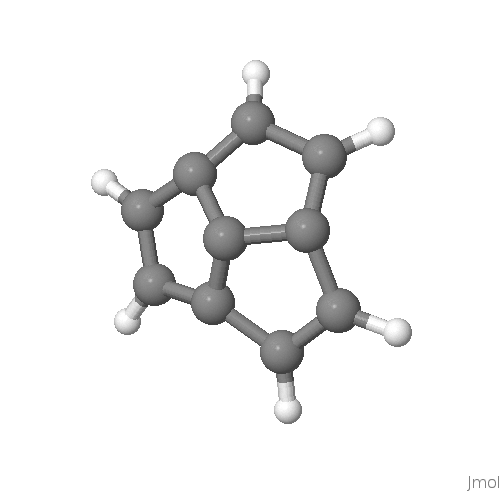
\includegraphics[scale=0.5]{M10001.png}\\


\captionof{table}{Singlet triplet gap} \label{tab:title} 
\begin{tabular}{c c c c}
\iffalse
CAMB3LYP & cc-pVTZ & -384.393573215265 & Singlet\\
CAMB3LYP & cc-pVTZ & -384.387733897973 & triplet\\
\fi
CAMB3LYP & cc-pVTZ & -0.15889599 eV & singlet triplet gap\\
\iffalse
SFTDDFT & cc-pVTZ & -384.36776641 & singlet\\
SFTDDFT & cc-pVTZ & -384.35641075 & triplet\\
\fi
SFTDDFT & cc-pVTZ & -0.3090034065 eV & singlet triplet gap\\
\iffalse
    B3LYP & cc-pVTZ & -384.61973856892 & Singlet \\
    B3LYP & cc-pVTZ & -384.61456371736 & triplet \\
\fi
    B3LYP & cc-pVTZ & -0.14081495 eV & singlet-triplet gap \\
\iffalse
    CCSD & def2-svp & -382.40331251 & singlet\\
    CCSD & def2-svp & -382.41292179 & triplet\\
\fi
    CCSD & def2-svp & 0.2614819617921767 eV& singlet triplet gab\\
\iffalse
    EOM-CCSD & cc-pVTZ & -383.67973970 & singlet\\
    EOM-CCSD & cc-pVTZ & -383.66063530 & triplet\\
\fi
    EOM-CCSD & cc-pVTZ & -0.5198574701600912 eV & singlet triplet gap\\
\iffalse
    EOM-SF-CCSD & cc-pVTZ & -383.67927397 & singlet\\
    EOM-SF-CCSD & cc-pVTZ & -382.66063530 & triplet\\
\fi
   EOM-SF-CCSD & cc-pVTZ & -0.5198574701600912 eV & singlet triplet gap\\ 
\iffalse
    CASSCF & cc-pVTZ & -382.18325411 & singlet\\
    CASSCF & cc-pVTZ & -382.14901925 & triplet\\
\fi
    CASSCF & cc-pVTZ & -0.9315784694047184 eV & singlet triplet gap\\
\iffalse
    CASPT2 & cc-pVTZ & -383.6944343574 & singlet\\
    CASPT2 & cc-pVTZ & -383.6586533857 & triplet\\
\fi
    CASPT2 & cc-pVTZ & -0.9736503333167863 eV & singlet triplet gap\\
\end{tabular}\\*

There are 66 electrons and 384 basis function when cc-pVTZ basis set is used. where as 190 basis function when def2-svp basis set is used. The singlet and the triplet geometry converged to structures which have energy of 384 \(\pm\) 1 Hartree. From the DFT calculations singlet and triplet is -0.158 ev. Which suggests that the singlet is the ground state. But CCSD calculation suggest that the molecule with triplet configuration is the ground state. CASSCF calculation done by bagel software package. 
In EOM-CCSD calculation 10 orbitals were taken to be frozen, 23 active occupied orbital and 351 active virtual orbital were considered for the calculation. In calculation for singlet configuration the molecular structure whose geometry is optimised for singlet configuration is taken as the reference for EOM-CCSD, where as the singlet configuration of the molecular structure optimised for triplet configuration is taken as the reference for EOM-CCSD as the EOM-CCSD calculation can only be performed with closed-shell restricted reference. 4 singlet and triplet excited state root were calculated in the respective molecule.
In the singlet calculation the total CCSD energy came out to be -383.67973970 hartree  with \( T _{1}^{2} = 0.0165\) \(T _{2}^{2} = 0.5946 \). A detail information of excitation of singlet structure is given in the table below

\captionof{table}{Singlet excitation EOM-SF-CCSD} \label{tab:title} 
\begin{tabular}{c c c c c c}
    State & Total Energy(a.u) & Excitation Energy (ev) & \(R_{0}^{2}\) & \(R_{1}^{2}\) & \(R_{2}^{2}\)\\
    First & -383.59635586 & 2.2690 & 0.0000 & 0.9155 & 0.0845 \\
    Second& -383.58017624 & 2.7093 & 0.0011 & 0.9158 & 0.0842 \\
    Third & -383.50290582 & 4.8119 & 0.0000 & 0.8965 & 0.1035 \\
    Forth & -383.50283661 & 4.8138 & 0.0000 & 0.8993 & 0.1007 \\
\end{tabular}\\*
In EOM-CCSD calculation of the triplet structure the total CCSD energy of the reference structure in singlet configuration was -383.63328048 hartree with \( T _{1}^{2} = 0.0324\) \(T _{2}^{2} = 0.5917 \). This configuration is excited to triplet state. The detailed information of the excitation to various triplet configuration is give in the table below.

\captionof{table}{Triplet EOM-SF-CCSD} \label{tab:title} 
\begin{tabular}{c c c c c c }
State & Total Energy(a.u) & Excitation Energy (ev) & \(R_{0}^{2}\) & \(R_{1}^{2}\) & \(R_{2}^{2}\)\\
First & -383.66063530&   -0.7444 & 0.0000 & 0.9236 & 0.0764 \\
Second& -383.61352826&   0.5375 & 0.0000 & 0.9198 & 0.0802 \\
Third & -383.53654527&   2.6323 & 0.0000 & 0.9335 & 0.0665 \\
Forth & -383.53364440&   2.7112 & 0.0000 & 0.9074 & 0.0926 \\
\end{tabular}
The negative value of the excitation energy shows that the triplet configuration is lower for this structure.

In the spin flip dft 4 excited states were calculated. For this calculation the triplet configuration of the singlet optimised structure was taken as reference for excitation and viceversa for the triplet optimised structure. Its description is as follows:


\captionof{table}{Singlet SFTDDFT} \label{tab:title} 
\begin{tabular}{c c c c}
State  & Excitation Energy(ev) & Total Energy(a.u) & \(\langle S^{2}\rangle \)\\
First  &  -0.8420           & -384.36776641 au      & 0.1041\\
Second &   0.4172           & -384.32149104 au      & 2.0245\\
Third  &   0.9790           & -384.30084678 au      & 0.1967\\
Forth  &   1.1033           & -384.29627696 au      & 0.9998\\
\end{tabular}


Similarly in case of triplet system:


\captionof{table}{Triplet SFTDDFT} \label{tab:title} 
\begin{tabular}{c c c c}
State & Excitation energy(ev) & Total energy(a.u) & \(\langle S^{2} \rangle \)\\
First & -0.7111 & -384.35641075 & 2.0000\\
Second & 0.4929 & -384.31216538 &  2.0000\\
Third & 2.5877 & -384.23518097 & 2.0000\\
Forth & 2.7062 & -384.23082735 & 2.0000\\
\end{tabular}

In the above mention result table of spinflip DFT the first excitation has a negative value. which means that the first excited state is the ground state for the respective molecular structure in their respective configuration. Though It is visible that the \(\langle S^{2} \rangle\) value in the triplet configuration is 2.0 in ground as well in all the excited states. So there is no spin contamination in triplet configuration calculation where as in the calculation of singlet configuration spin contamination is visible.

Spin flip DFT with number of excited state set to be 10. The data for singlet is shown as follows


\captionof{table}{Singlet SFTDDFT 10 excitations} \label{tab:title} 
\begin{tabular}{c c c c}
State & Excitation energy(ev) & Total energy(a.u) & \(\langle S^{2} \rangle \)\\
First & -0.8420 & -384.36776640 & 0.1041\\
Second & 0.4172& -384.32149104 &2.0245\\
Third & 0.9790& -384.30084678 &0.1967\\
Forth & 1.1033& -384.29627697 &0.9999\\
Fifth & 2.0420& -384.26178179 &1.0059\\
Sixth & 2.5151& -384.24439671 &0.3119\\
Seventh & 3.2713& -384.21660491 &0.9882\\
Eighth & 3.4895& -384.20858736 &1.0504\\
Ninth & 4.1861& -384.18298580 &1.1203\\
Tenth & 4.4526& -384.17319386 &1.1304\\
\end{tabular}\\*

Data for triplet state is shown below


\captionof{table}{Triplet SFTDDFT 10 excitations} \label{tab:title} 
\begin{tabular}{c c c c}
State & Excitation energy(ev) & Total energy(a.u) & \(\langle S^{2} \rangle \)\\
First & -0.7111& -384.35641075 & 2.0000\\
Second &0.4929 & -384.31216538 & 2.0000\\
Third & 2.5877 & -384.23518097 & 2.0000\\
Forth & 2.7062 & -384.23082735 & 2.0000\\
Fifth & 3.7755& -384.19153089 & 2.0000\\
Sixth & 4.4644& -384.16621508 & 2.0000\\
Seventh & 4.6699 & -384.15866262 & 2.0000\\
Eighth &4.7376 & -384.15617318 & 2.0000\\
Ninth & 4.8994& -384.15022698 & 2.0000\\
Tenth &4.9884&-384.14695619 & 2.0000\\
\end{tabular}

As the number of excited state was increased the singlet triple gap became -0.30900313440957844 ev. The difference of singlet triplet gap \(2.7209042158249^{-7}\)ev. From this data of excitation energy and the transition moment between the excited state the spectrum was calculated. In order to calculate the spectrum, The difference between the first excited state and rest of the excited state was calculated since the first excited state which happens to be the ground state in both of their respective configuration, and thus excitation energy from the ground state was calculated. From the qchem calculation data, the strength of the transition moment between first excited state and rest of the excited state of SFTDDFT calculation was used for calculation of oscillator strength. 

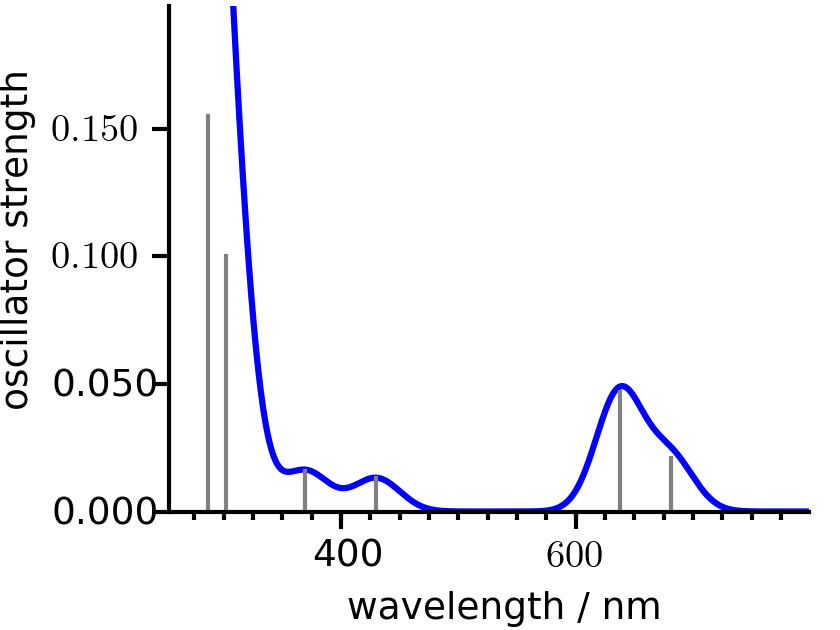
\includegraphics[scale=0.5]{M1_sin_sfdft_spec.png}\\
For further investigation done by CASSCF method. CASSCF was performed using bagel software package. The calculation was performed selecting various kind of active space, Their description is given below. In the hartree-Fock calculation 33rd orbital happens to be the highest occupied molecular orbital. For calculation involving active space with 4 orbitals only 2 electron was taken into account and 4 states were considered for state averaging calculation. After estimating the computational time the calculation would utilize. Further calculation were performed using 6 electrons and 6 8 and 10 orbitals for both singlet and triplet structures.In the table below the zeropoint energy of the lowest state in state averaging calculation has been report. From the calculation involing 10 orbital in active space natural orbital occupation number of both the structures is reported in the table 9 and 10.

\captionof{table}{CASSCF} \label{tab:title} 
\begin{tabular}{c c c c}
active space& Singlet Energy &Triplet Energy & singlet triplet difference\\
4 & -382.09583002 & -382.08958442 & -0.16995151983999293\\
6 & -382.16664933 & -382.14941603 & -0.46894221961963767\\
8 & -382.17663273 & -382.14388369 & -0.891147227055967\\
10 & -382.18325411& -382.14901925 & -0.9315784694047184\\
\end{tabular}\\*
Natural Orbital Occupation Number of Singlet optimised molecule of the orbital in active space  \\*

\captionof{table}{NOONs singlet} \label{tab:title} 
\begin{tabular}{c c}
Orbital 31 & 1.8917\\
Orbital 32 & 1.6083\\
Orbital 33 & 1.3069\\
Orbital 34 & 0.9788\\
Orbital 35 & 0.0956\\
Orbital 36 & 0.0778\\
Orbital 37 & 0.0171\\
Orbital 38 & 0.0154\\
Orbital 39 & 0.0044\\
Orbital 40 & 0.0040\\
\end{tabular}\\
Natural  Orbital Occupation of triplet state of the orbital in active space\\*

\captionof{table}{NOONS triplet} \label{tab:title} 
\begin{tabular}{c c}
Orbital 31 & 1.7557\\
Orbital 32 & 1.4502\\
Orbital 33 & 1.3198\\
Orbital 34 & 1.2079\\
Orbital 35 & 0.1333\\
Orbital 36 & 0.0814\\
Orbital 37 & 0.0327\\
Orbital 38 & 0.0126\\
Orbital 39 & 0.0036\\
Orbital 40 & 0.0027\\
\end{tabular}

Further geometry optimization calculation was performed using CASSCF method in triplet configuration and Structure converged to geometry having -382.18555754 hartree. which is lower than the energy of the singlet structure.


Later on CASPT2 calculation was performed on the molecular structures with 10 orbitals in active space and 4 states were chosen for state averaging. The singlet triplet gap from the calculation has been reported in the table 


Bond distance of the central carbon from the neighbouring carbon of the singlet structure(in Angstrom)\\*


\begin{tabular}{c c}
\(c^{*}-c^{1}\) & 1.43989 \\
\(c^{*}-c^{2}\) & 1.43939 \\
\(c^{*}-c^{3}\) & 1.34563 \\
\end{tabular}\\*
Bond angle of the central carbon from the neighbouring carbon of the singlet structure (in degree)\\*

\begin{tabular}{c c}
\(c^{1}-c^{*}-c^{2}\) & 111.004\\
\(c^{2}-c^{*}-c^{3}\) & 111.004\\
\(c^{3}-c^{*}-c^{1}\) & 113.229\\
\end{tabular}\\*
Bond distance of the central carbon from the neighbouring carbon of the triplet structure(in Angstrom)\\*

\begin{tabular}{c c}
\(c^{*}-c^{1}\) 1.39801 \\
\(c^{*}-c^{2}\) 1.39803 \\
\(c^{*}-c^{3}\) 1.39804 \\
\end{tabular}\\*
Bond angle of the central carbon from the neighbouring carbon of the triplet structure (in degree)\\*

\begin{tabular}{c c}
\(c^{1}-c^{*}-c^{2}\) & 110.639 \\
\(c^{2}-c^{*}-c^{3}\) & 110.659 \\
\(c^{3}-c^{*}-c^{1}\) & 110.659 \\
\end{tabular}\\*
From the above data the triplet structure is more closed to the symmetric structure. 
Deviation of distance is 0.0937 Angstrom and angle is 2.2224 degree in singlet structure where as in triplet structure deviation of distance is 0.00001 Angstrom and of angle is 0.02 degree.\\*

\captionof{table}{Electron density map of Hartree Fock Orbitals that were chosen for active space of CASSCF of Singlet structure} \label{tab:title} 
\begin{tabular}{|c|c|}
\hline Orbital Number& image\\\hline
31 & 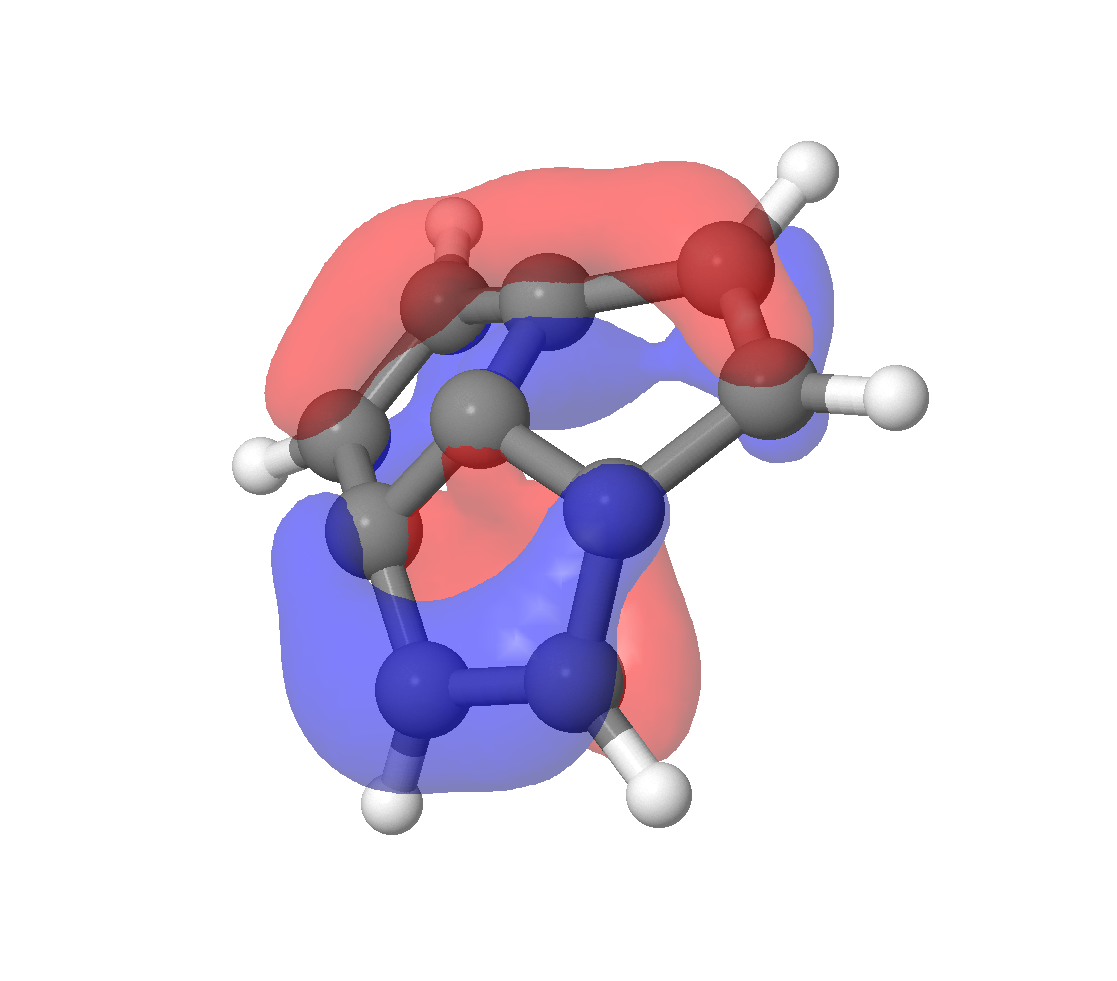
\includegraphics[scale=0.3]{M1S_31.png}\\ \hline
32 & 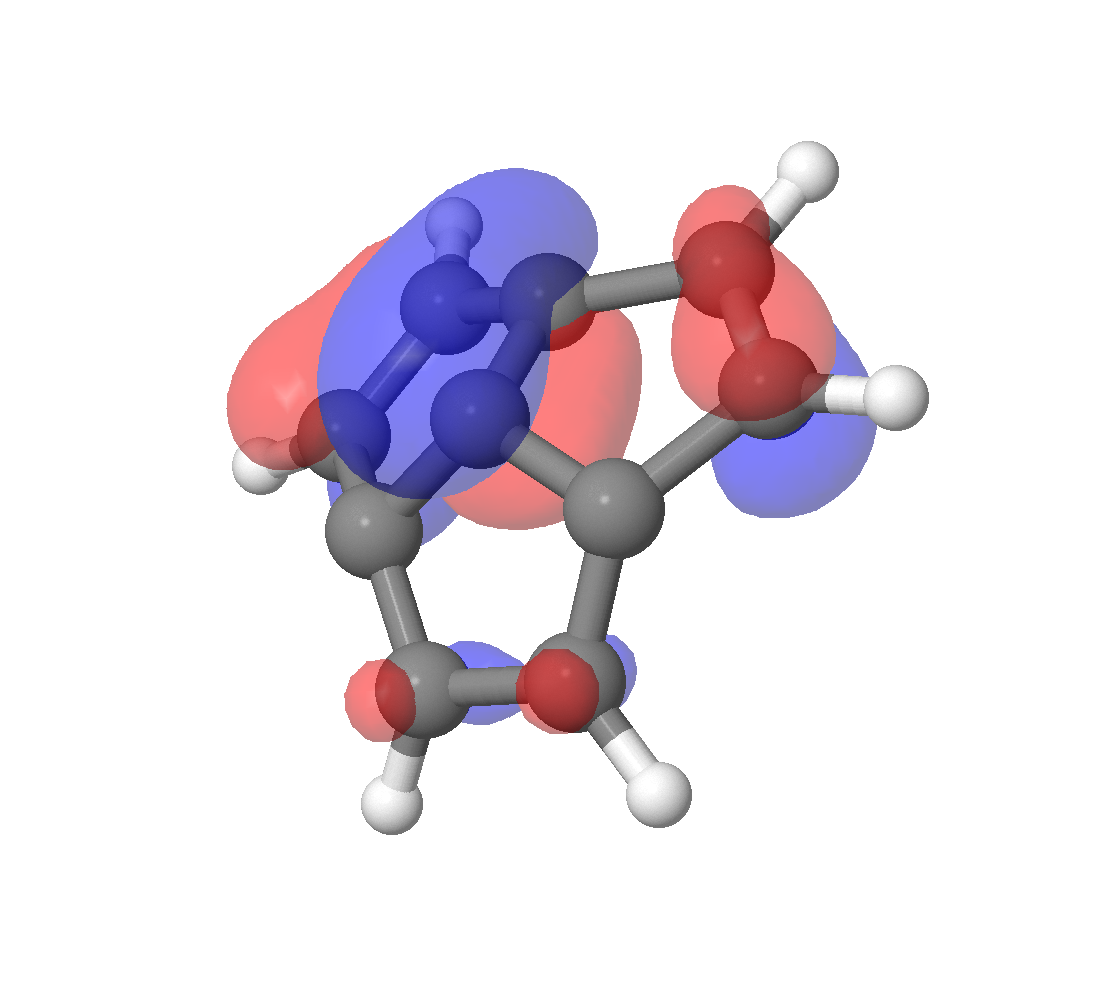
\includegraphics[scale=0.3]{M1S_32.png}\\ \hline
33 & 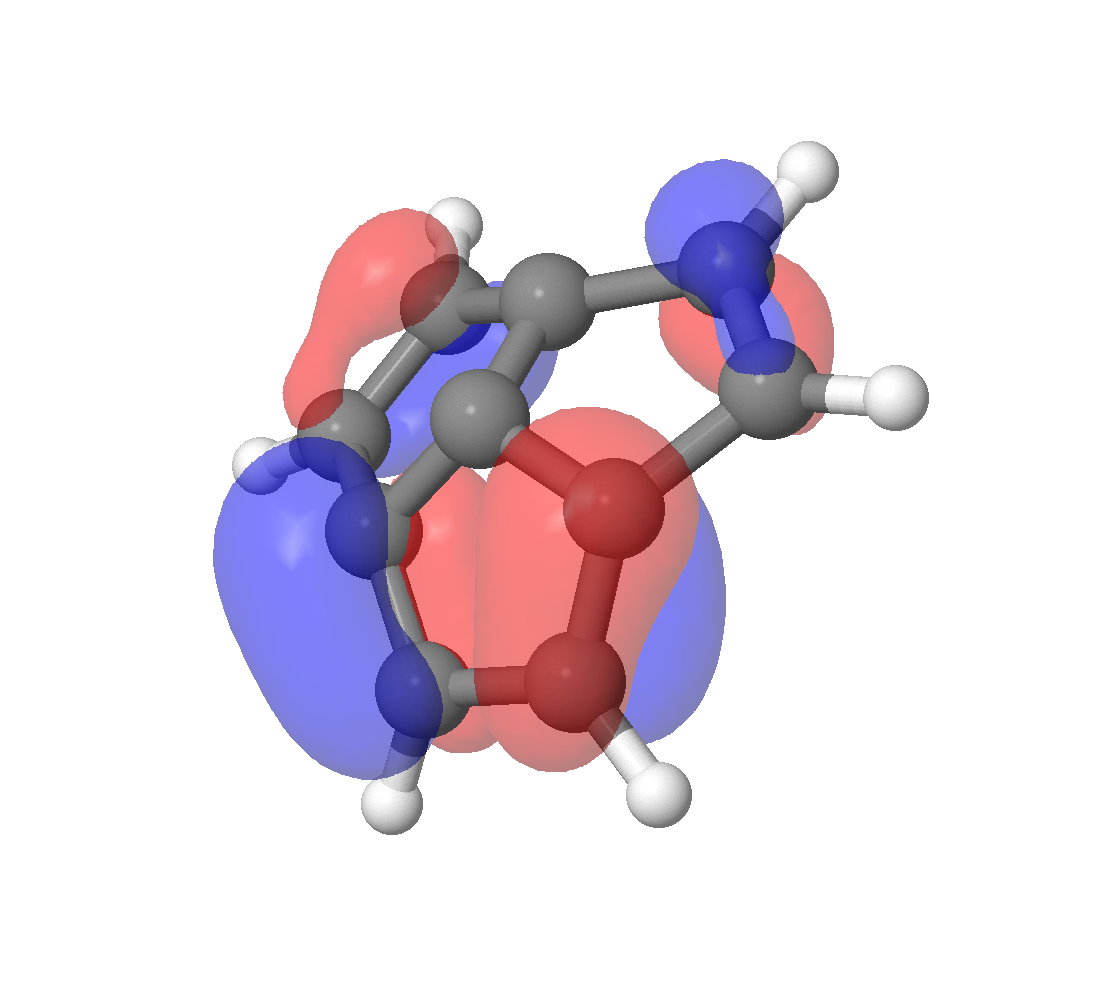
\includegraphics[scale=0.3]{M1S_33.png}\\ \hline
34 & 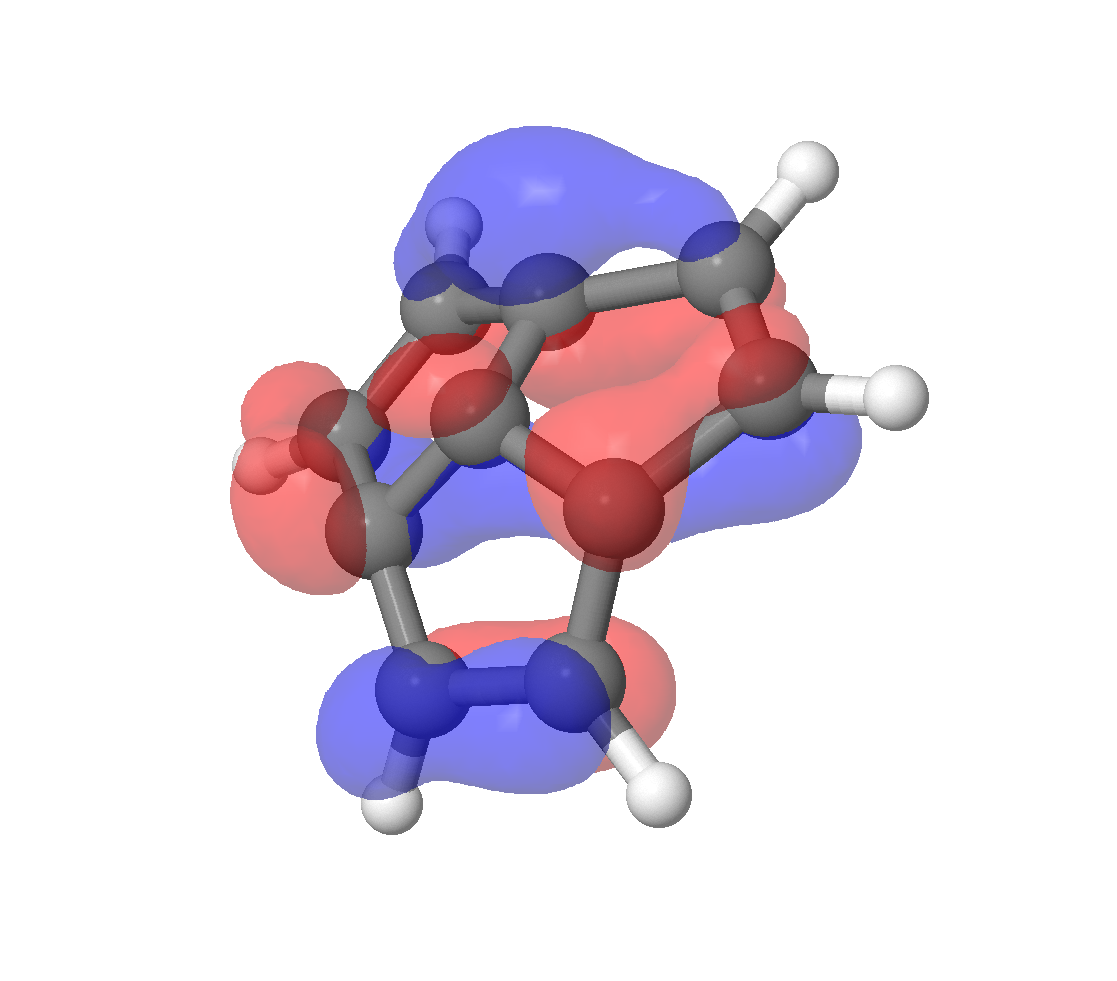
\includegraphics[scale=0.3]{M1S_34.png}\\ \hline
35 & 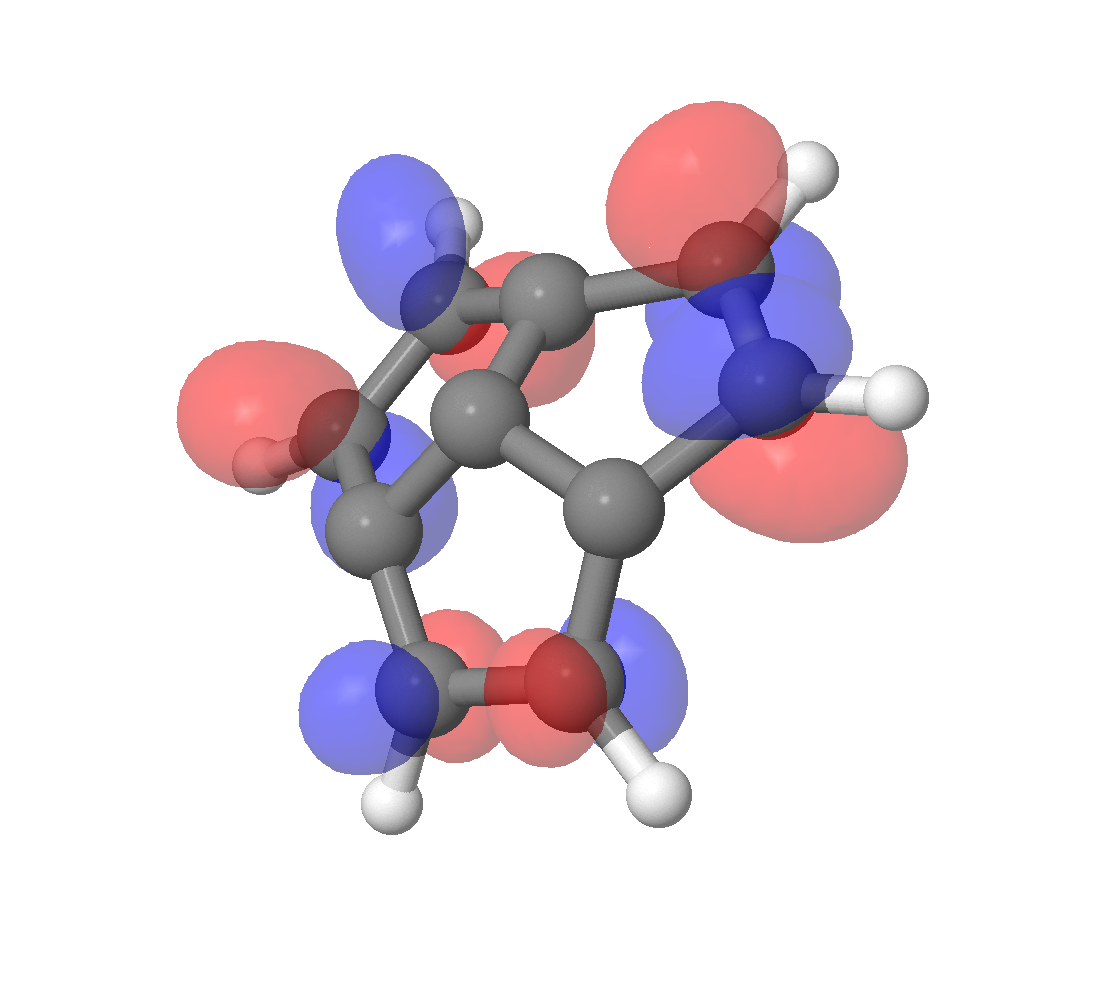
\includegraphics[scale=0.3]{M1S_35.png}\\ \hline
\end{tabular}
\begin{tabular}{|c|c|}
\hline Orbital Number& image\\\hline
36 & 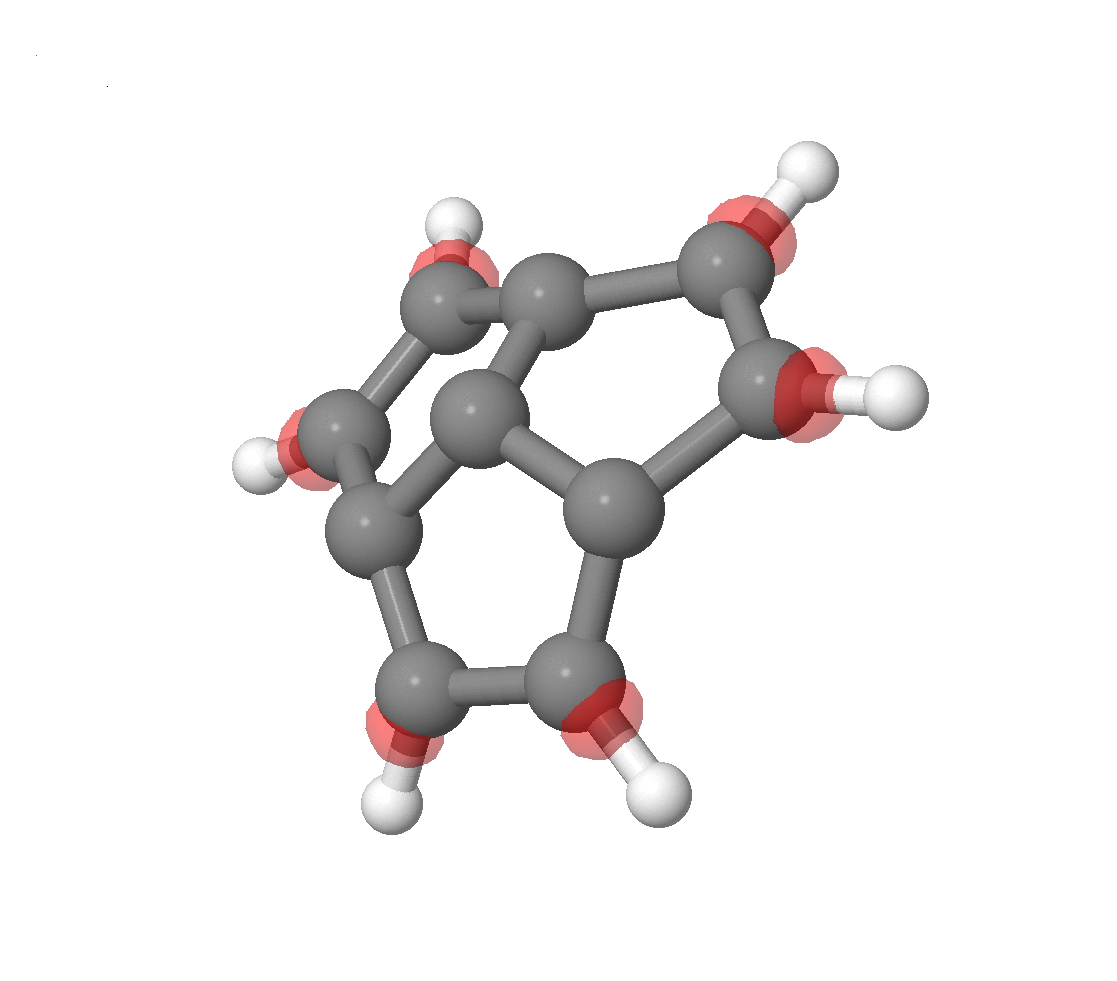
\includegraphics[scale=0.3]{M1S_36.png}\\ \hline
37 & 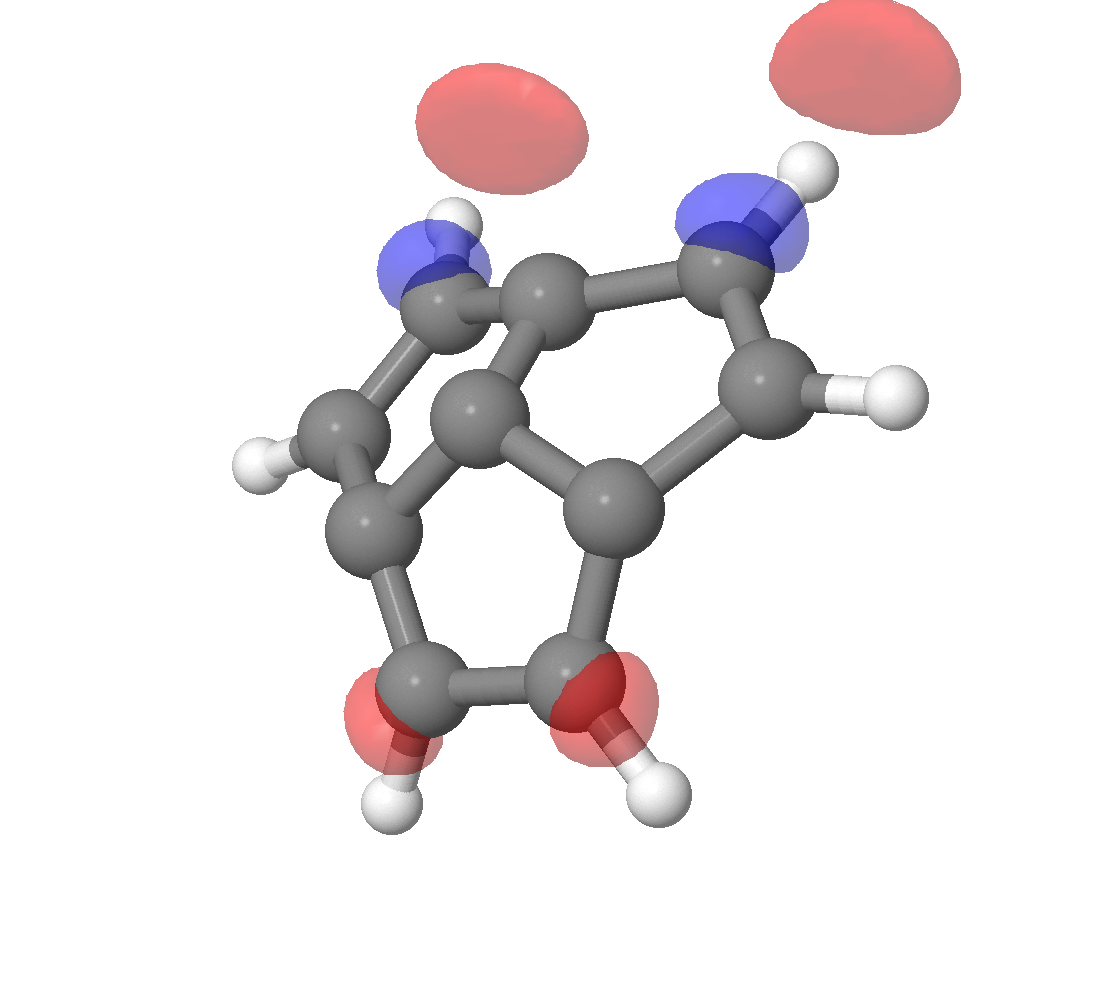
\includegraphics[scale=0.3]{M1S_37.png}\\ \hline
38 & 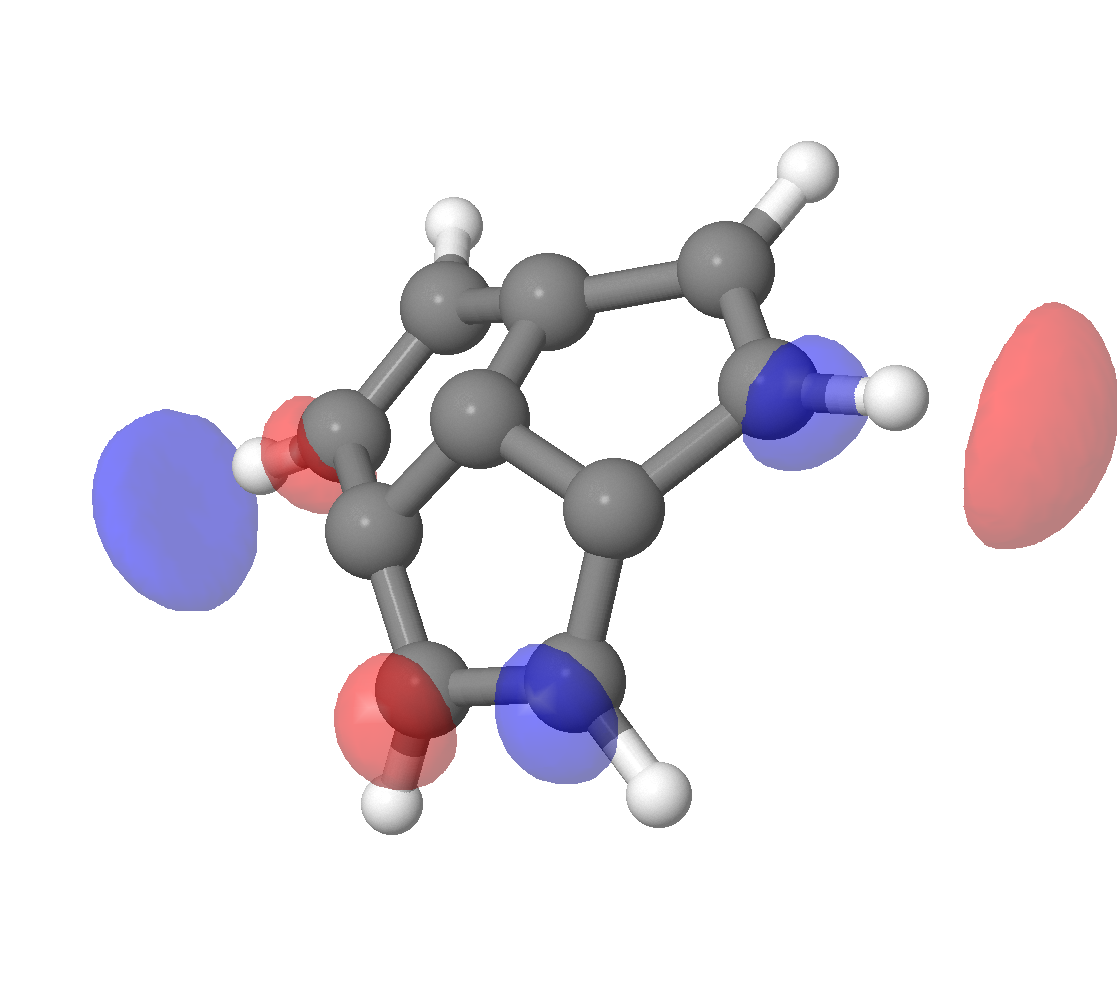
\includegraphics[scale=0.3]{M1S_38.png}\\ \hline
39 & 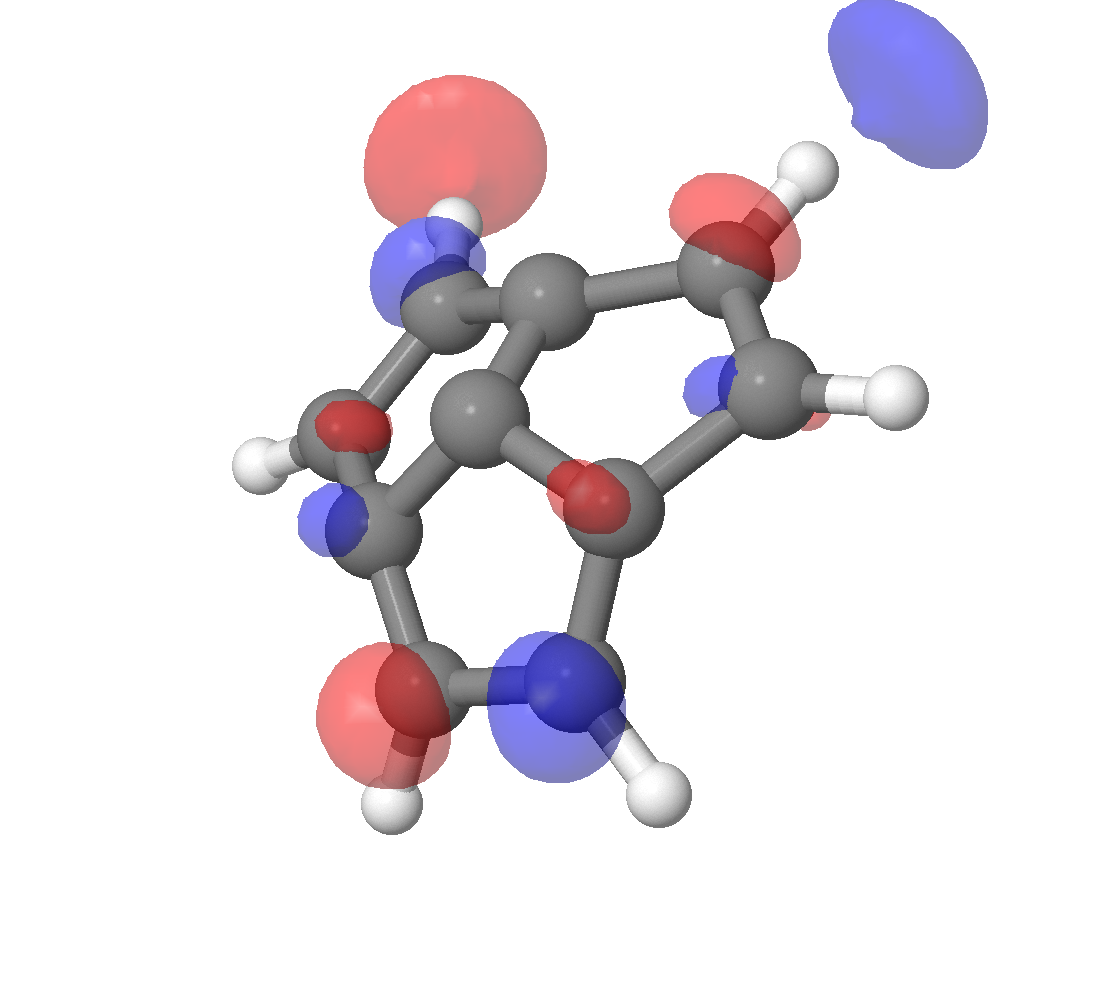
\includegraphics[scale=0.3]{M1S_39.png}\\ \hline
40 & 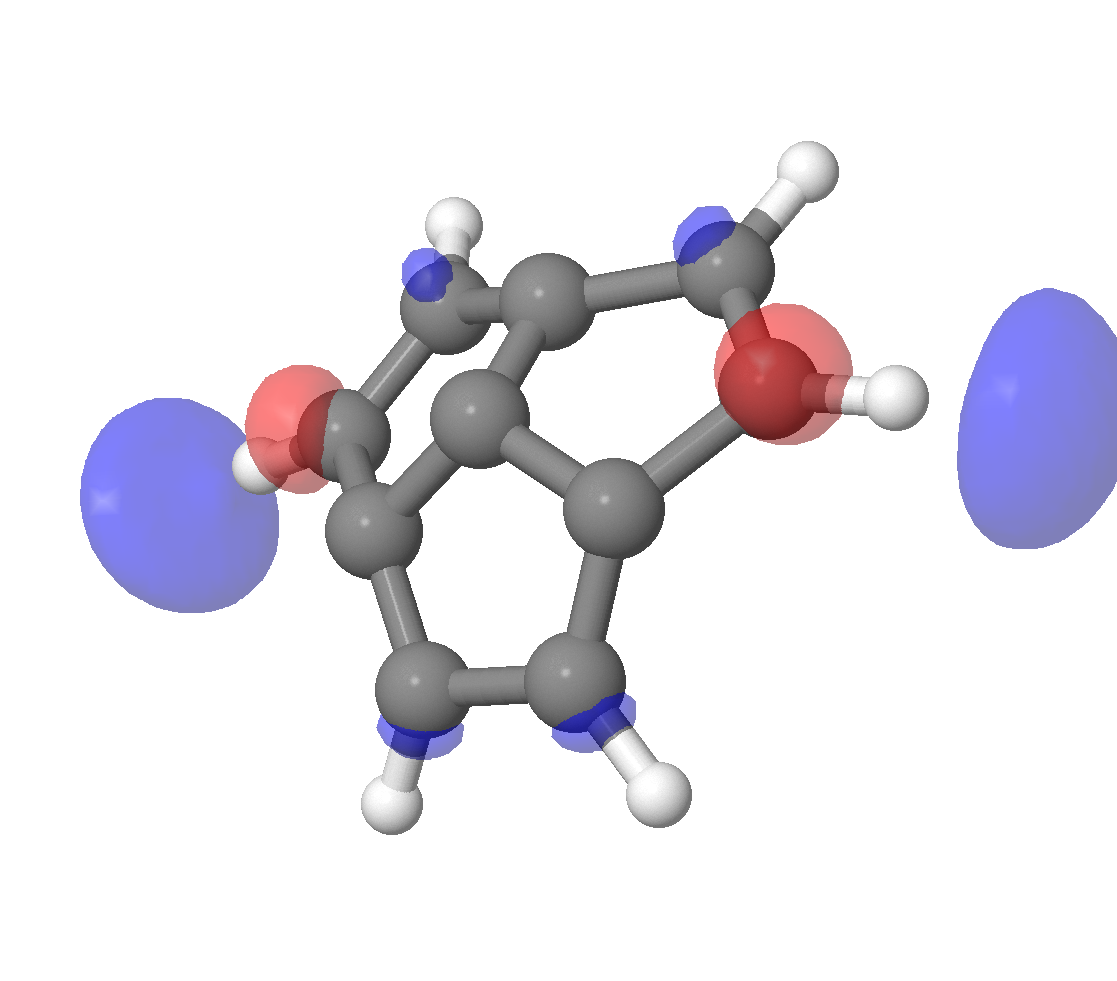
\includegraphics[scale=0.3]{M1S_40.png}\\ \hline
\end{tabular}
\\*
\captionof{table}{Hartree Fock Orbitals in active space of CASSCF of Triplet structure} \label{tab:title} 
\begin{tabular}{|c|c|}
\hline Orbital Number& image\\\hline
31 & 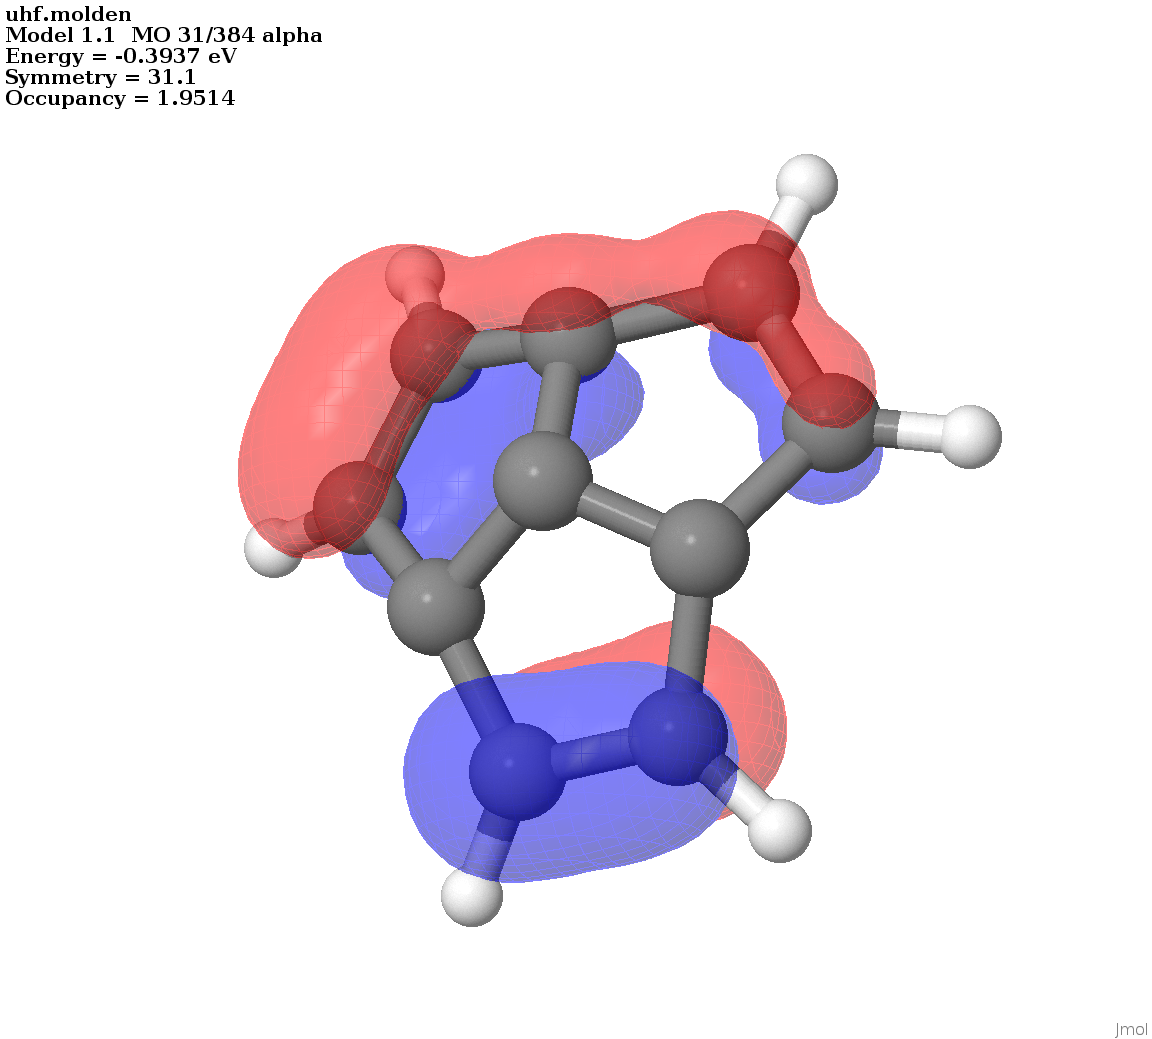
\includegraphics[scale=0.1]{M1T_31.png}\\ \hline
32 & 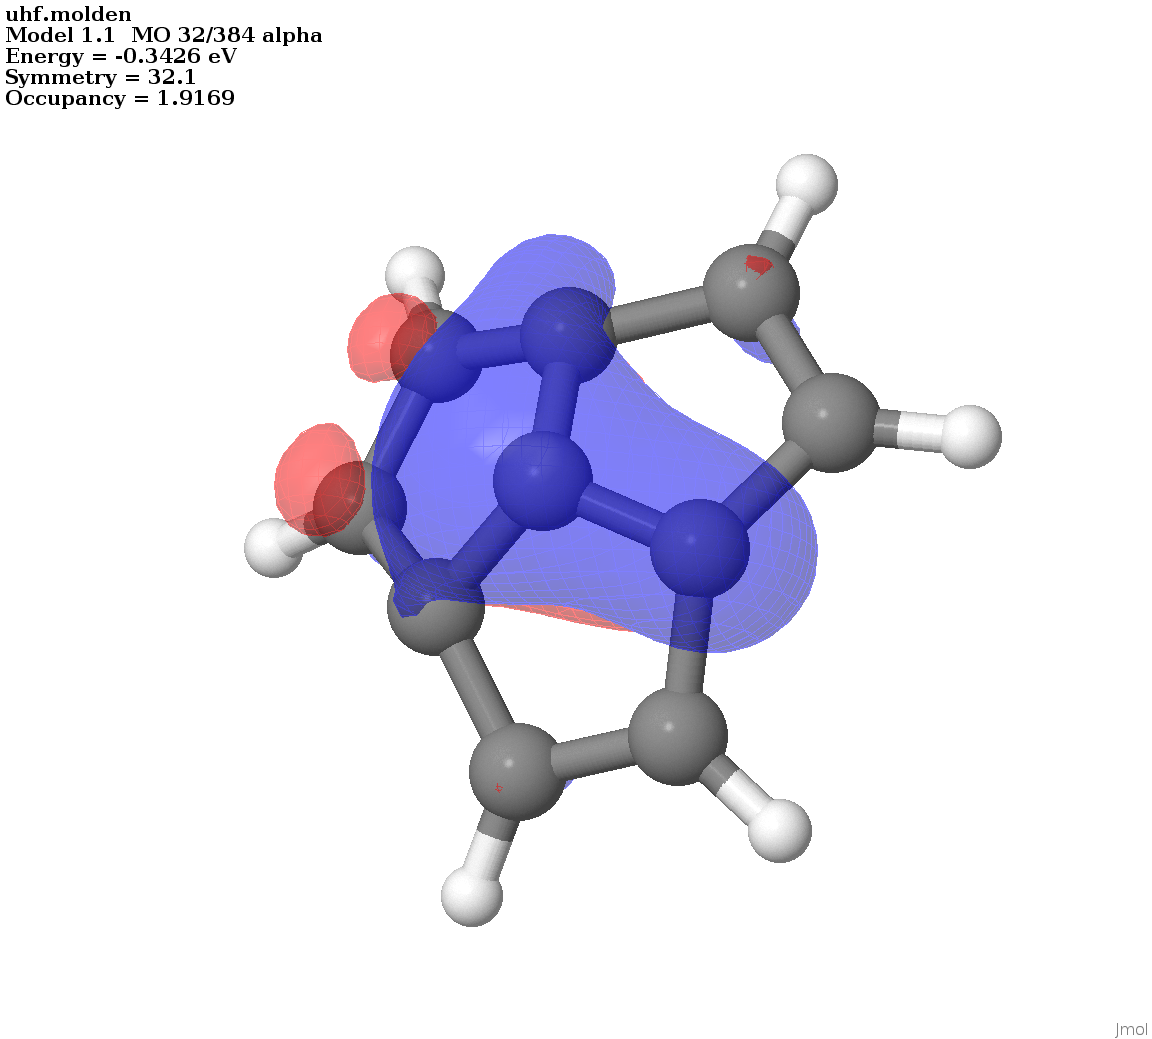
\includegraphics[scale=0.1]{M1T_32.png}\\ \hline
33 & 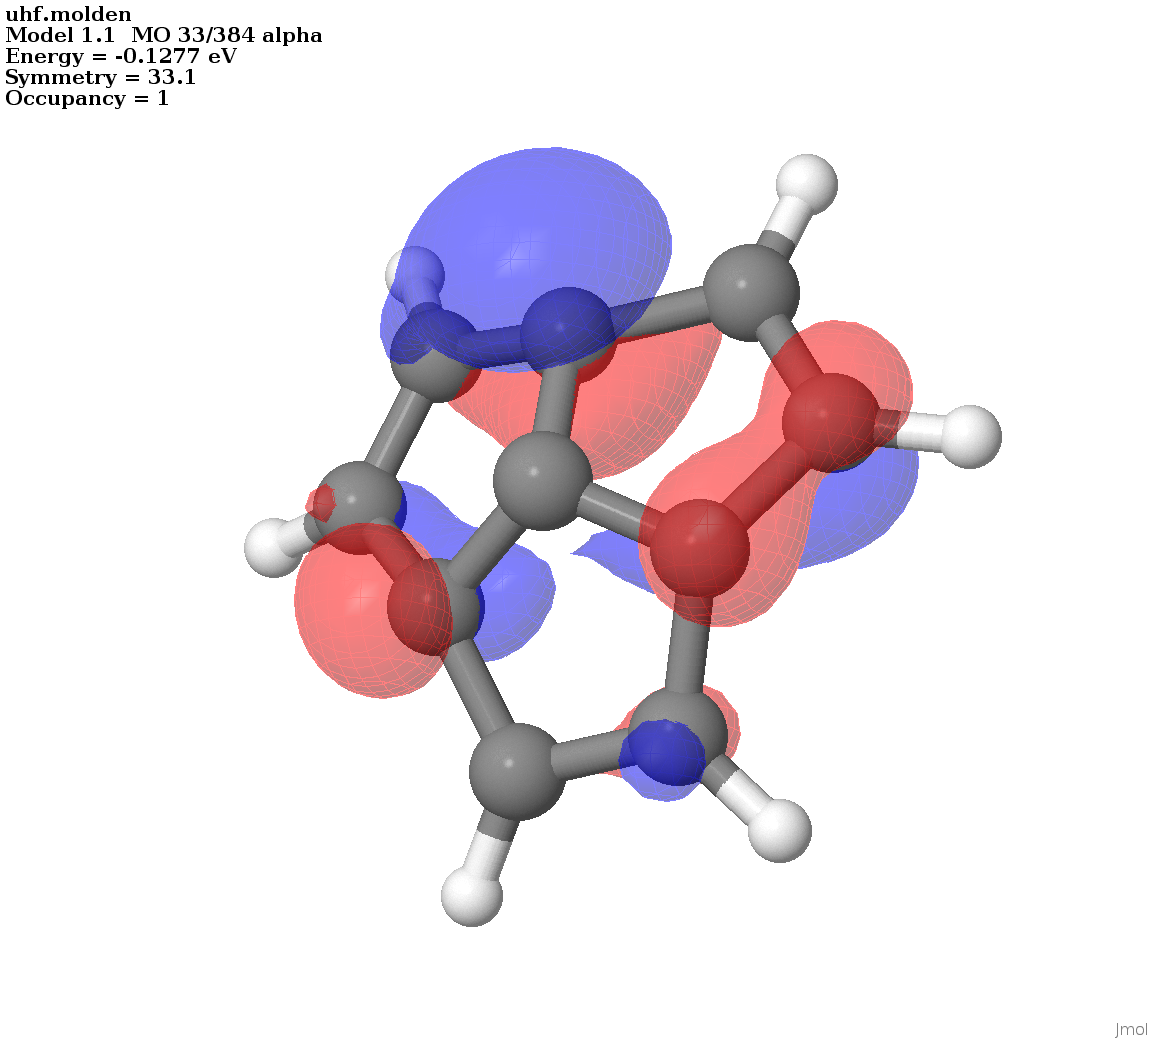
\includegraphics[scale=0.1]{M1T_33.png}\\ \hline
34 & 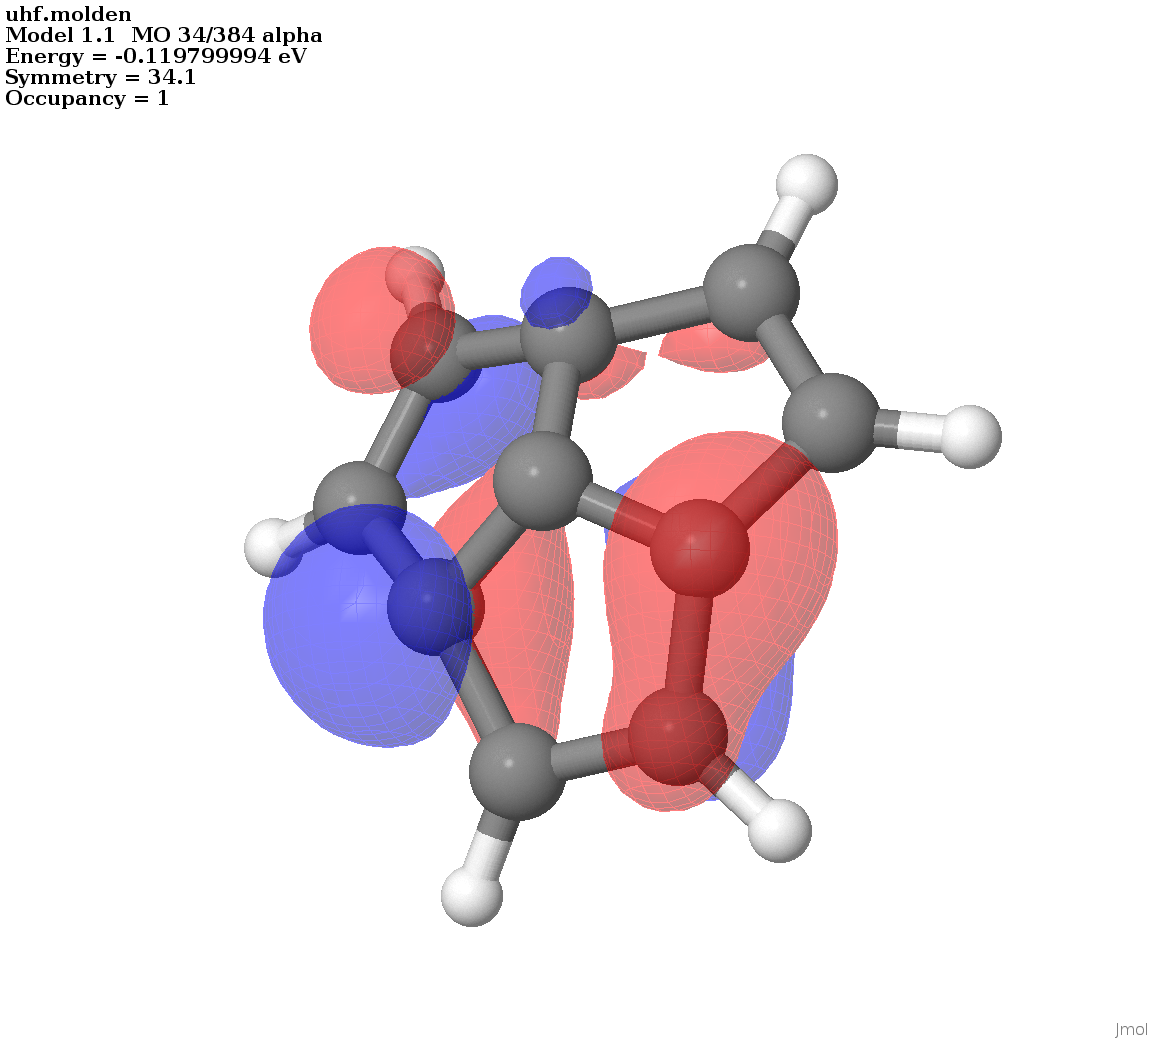
\includegraphics[scale=0.1]{M1T_34.png}\\ \hline
35 & 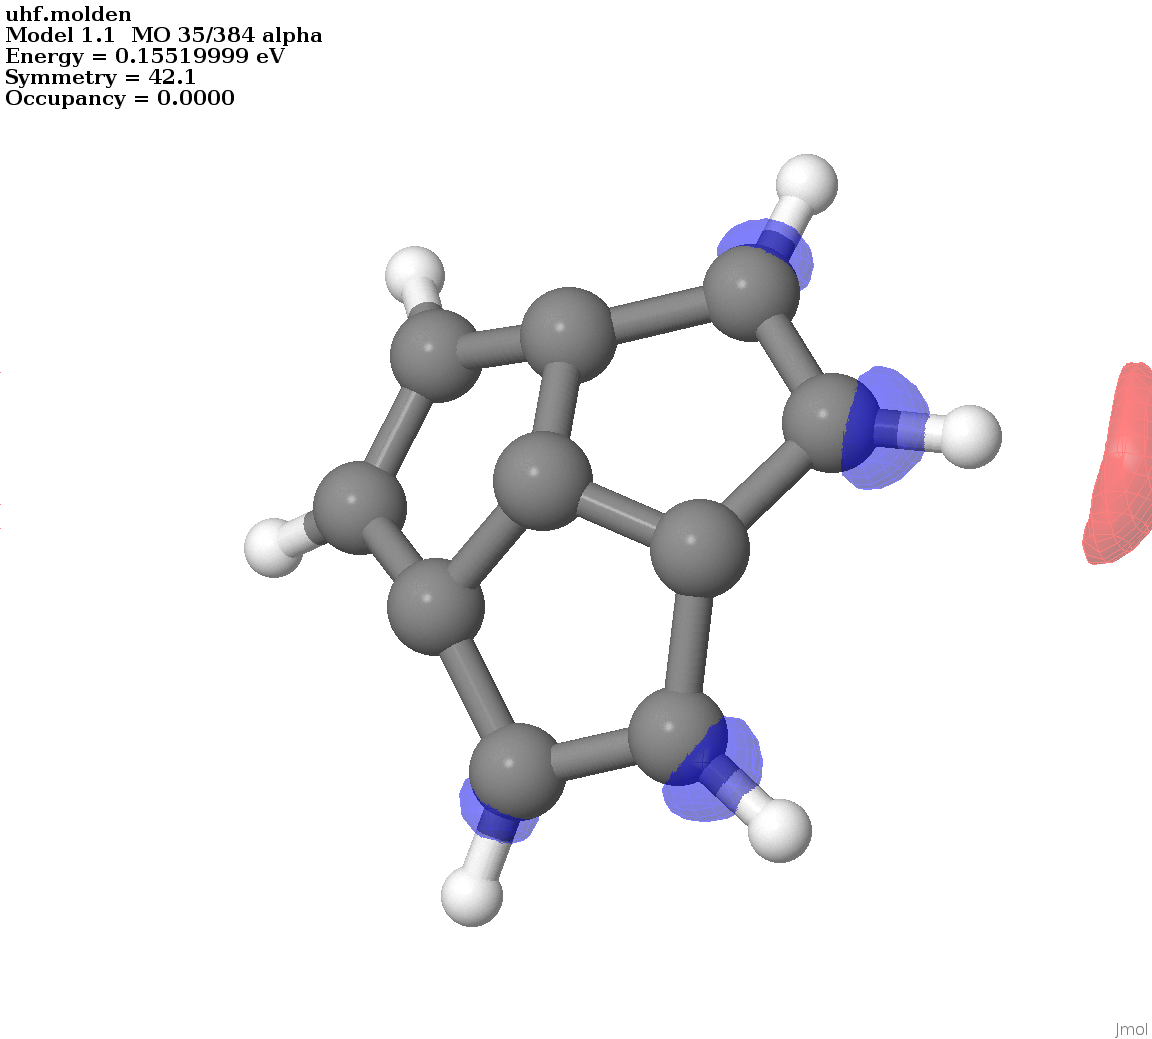
\includegraphics[scale=0.1]{M1T_35.png}\\ \hline
\end{tabular}
\begin{tabular}{|c|c|}
\hline Orbital Number& image\\\hline
36 & 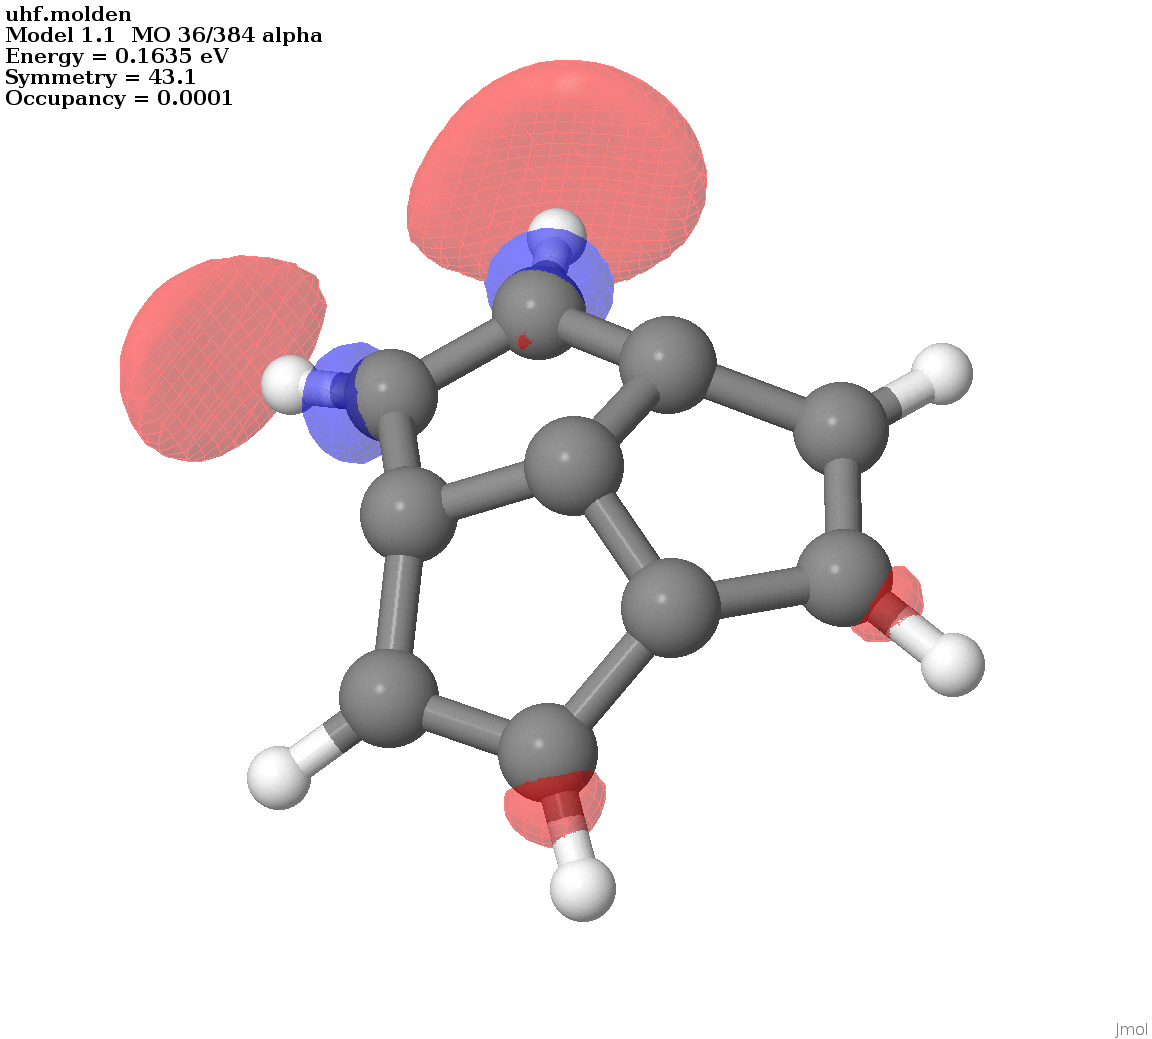
\includegraphics[scale=0.1]{M1T_36.png}\\ \hline
37 & 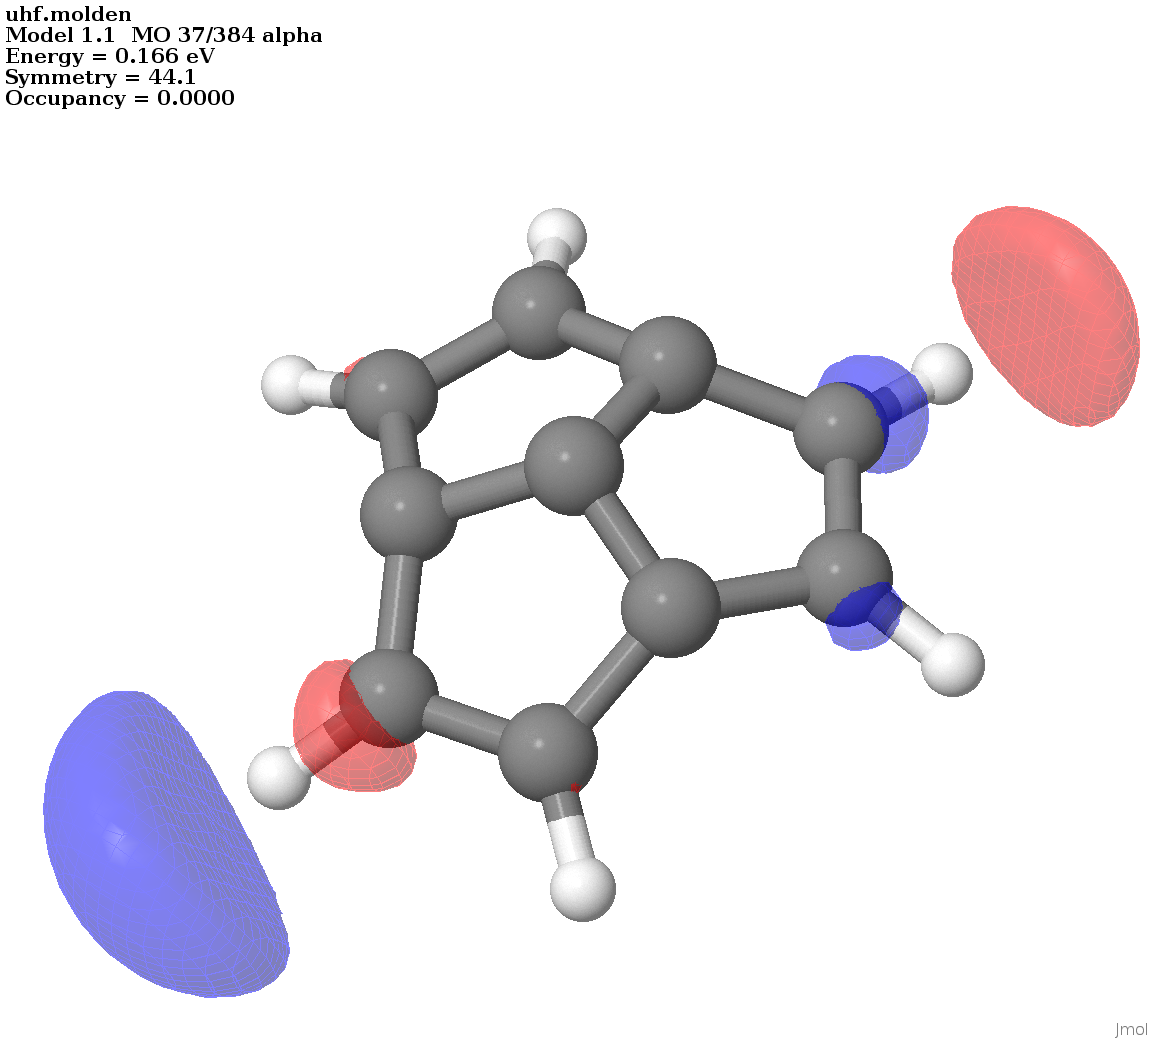
\includegraphics[scale=0.1]{M1T_37.png}\\ \hline
38 & 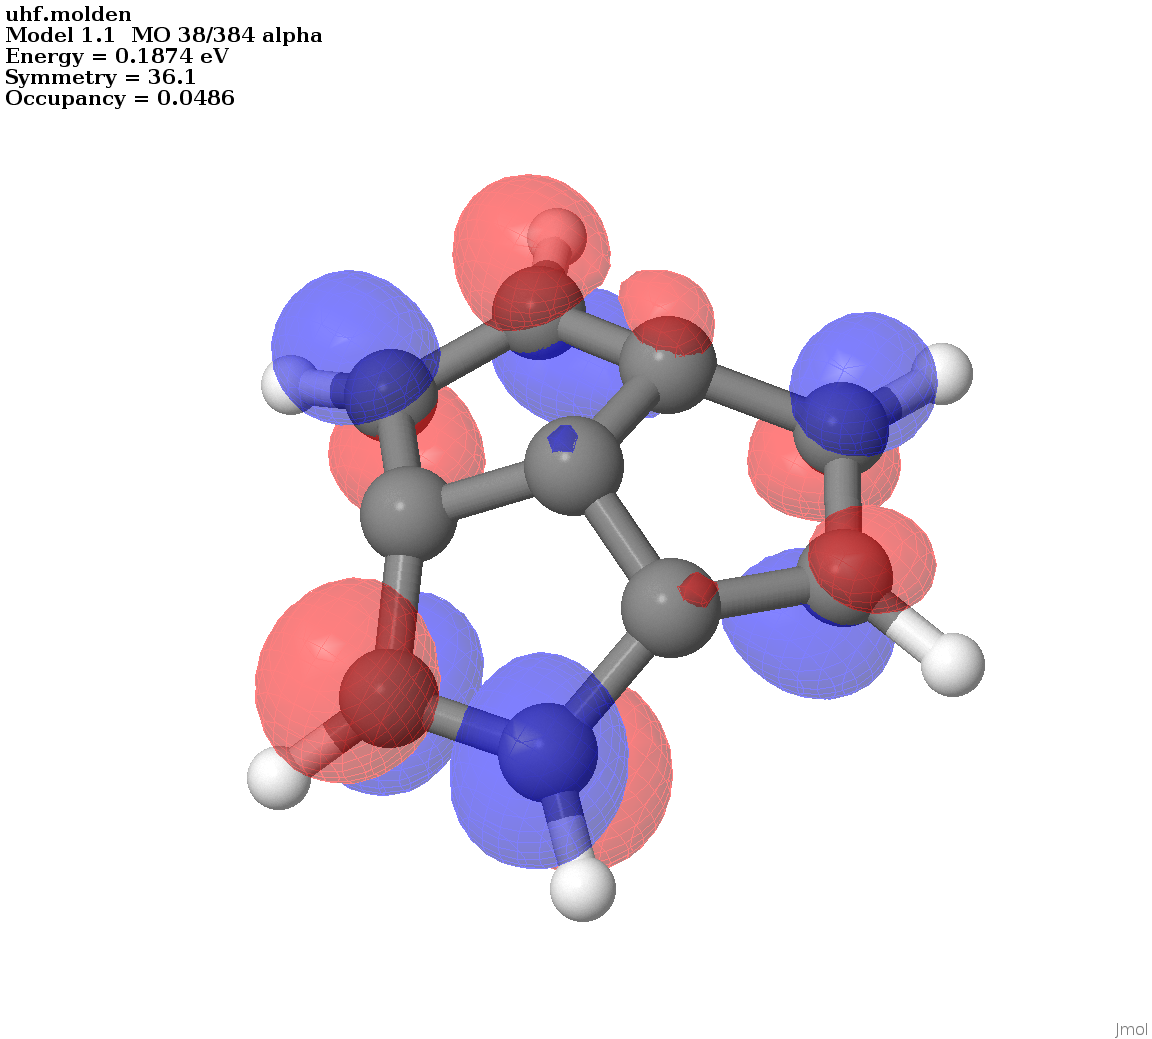
\includegraphics[scale=0.1]{M1T_38.png}\\ \hline
39 & 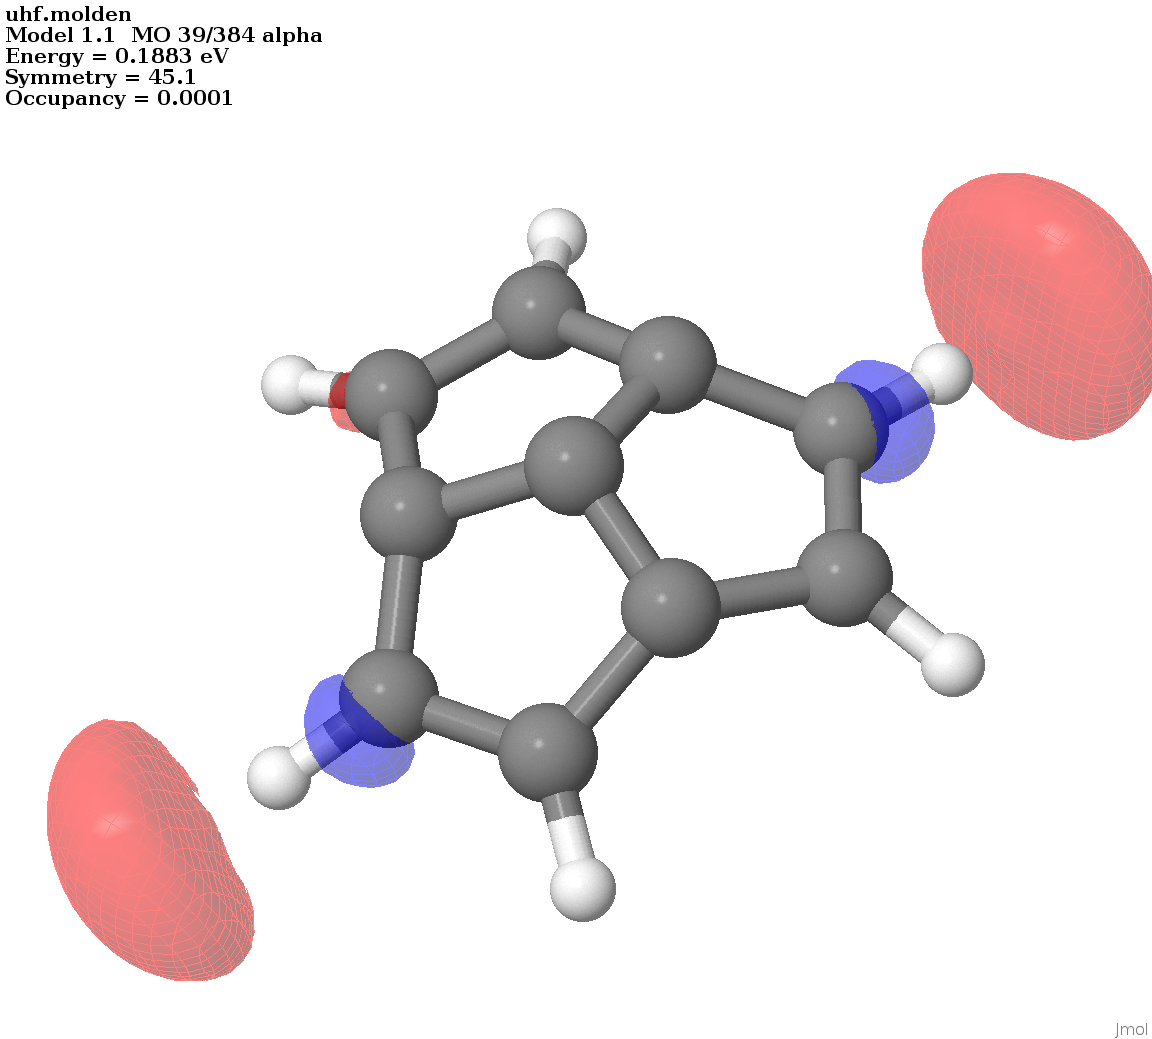
\includegraphics[scale=0.1]{M1T_39.png}\\ \hline
40 & 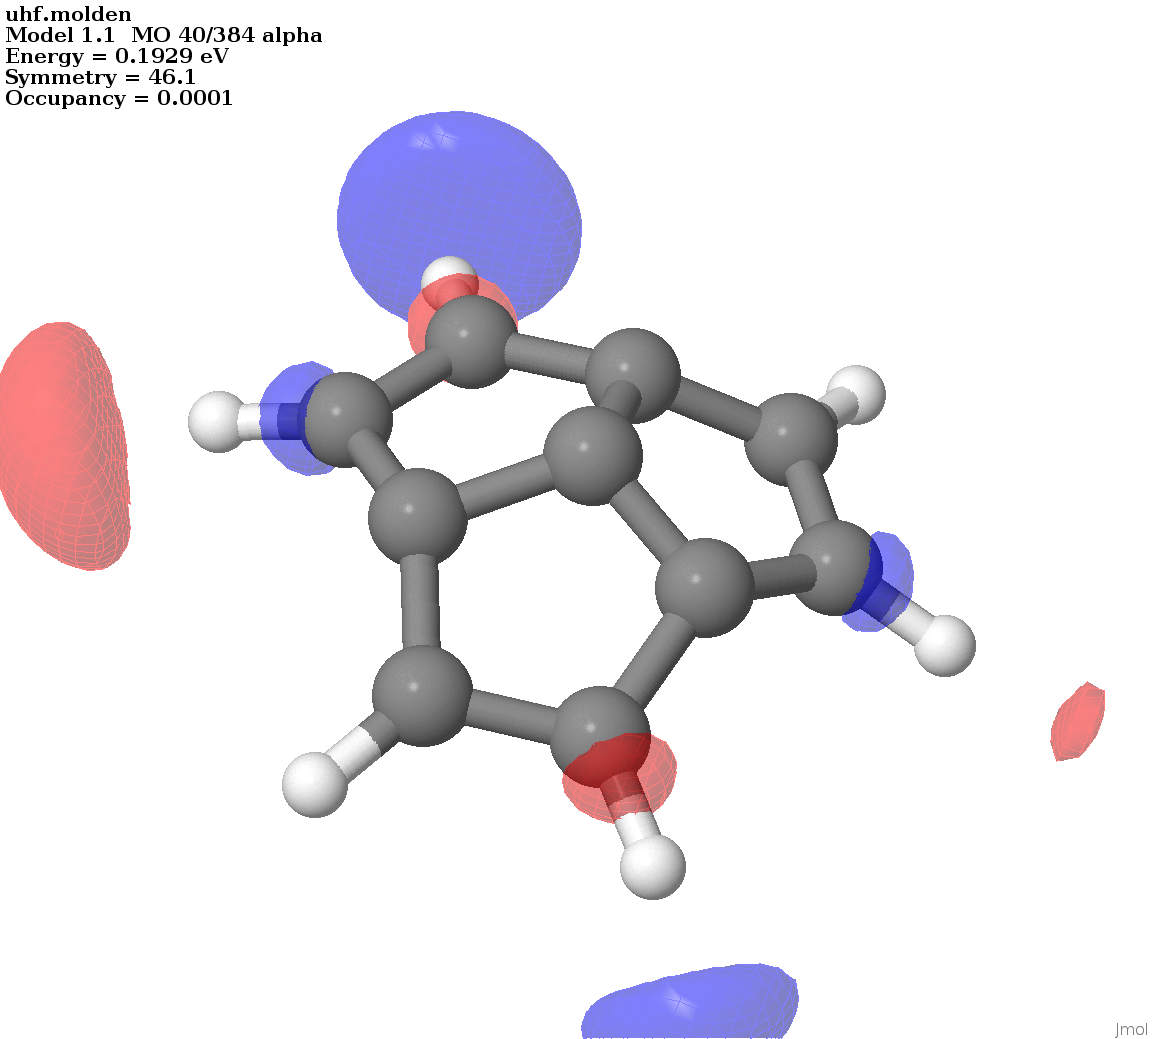
\includegraphics[scale=0.1]{M1T_40.png}\\ \hline
\end{tabular}
\iffalse
\iffalse
############################################################################
#
# Molecule 1 with 3 H
#
############################################################################
\fi
\pagebreak
\section{Molecule 1 With 4 H}

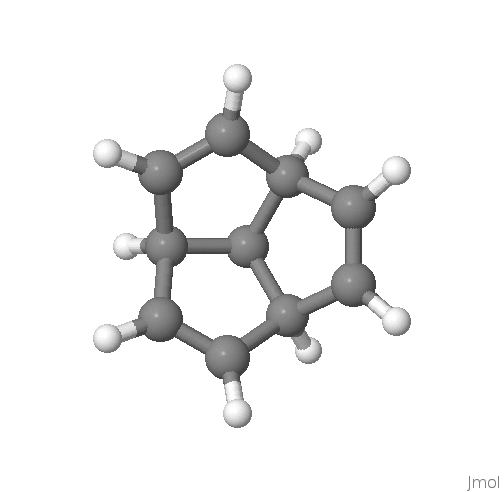
\includegraphics[scale=0.5]{M1_h_0001}\\

\begin{tabular}{c c c c}
\iffalse
SFTDDFT & cc_pVTZ & -386.89916333 & singlet\\
SFTDDFT & cc-pVTZ & -386.72233083 & triplet\\
\fi
SFTDDFT & cc-pVTZ & -4.81185989050125 & singlet triplet gap\\
\iffalse
CAMB3LYP & cc-pVTZ & -386.927595896334 & singlet\\
CAMB3LYP & cc-pVTZ & -386.802253894324 & triplet\\
\fi
CAMB3LYP & cc-pVTZ &  -3.41073135349571& singlet triplet gap\\
\iffalse
B3LYP & cc-pVTZ & -387.153580611325 & singlet\\
B3LYP & cc-pVTZ & -386.987965248093 & triplet\\
\fi
B3LYP & cc-pVTZ & -4.50662589505143 eV & singlet triplet\\
\iffalse
CCSD & def2-svp & -386.22016386 & singlet\\
CCSD & def2-svp & -386.19237203 & triplet\\
\fi
CCSD & def2-svp & -0.7562546028623374 & singlet triplet gap\\
\iffalse
EOM-CCSD & cc-pVTZ & -386.22016386 & singlet \\
EOM-CCSD & cc-pVTZ & -386.06635213  & triplet \\
\fi
EOM-CCSD & cc-pVTZ & -4.185432509722801 & singlet triplet gap\\
\iffalse
CASSCF & cc-pVTZ & -384.55180714 & singlet \\
CASSCF & cc-pVTZ & -384.34832904  & triplet \\
\fi
CASSCF & cc-pVTZ & -5.536923970339562 & singlet triplet gap\\
\end{tabular}\\*
There are 70 electrons and 440 basis function. Here the singlet structure have the lower energy than triplet structure. From the DFT calculation is inferred that 
hydrogen substituted acepentylene is not a biradical. because the singlet has the lower energy than the triplet one.
Bond distance of the central carbon from the neighbouring carbon of the singlet structure(in Angstrom)\\*
\begin{tabular}{c c}
\(c^{*}-c^{1}\) & 1.55122 \\
\(c^{*}-c^{2}\) & 1.55119 \\
\(c^{*}-c^{3}\) & 1.55122 \\
\end{tabular}\\*
Bond angle of the central carbon from the neighbouring carbon of the singlet structure (in degree)\\*
\begin{tabular}{c c}
\(c^{1}-c^{*}-c^{2}\) & 106.702\\
\(c^{2}-c^{*}-c^{3}\) & 106.696\\
\(c^{3}-c^{*}-c^{1}\) & 106.696\\
\end{tabular}\\*
Bond distance of the central carbon from the neighbouring carbon of the triplet structure\\*
\begin{tabular}{c c}
\(c^{*}-c^{1}\) 1.55566 nm\\
\(c^{*}-c^{2}\) 1.55217 nm\\
\(c^{*}-c^{3}\) 1.55566 nm\\
\end{tabular}\\*
Bond angle of the central carbon from the neighbouring carbon of the triplet structure (in degree)\\*
\begin{tabular}{c c}
\(c^{1}-c^{*}-c^{2}\) & 106.764 \\
\(c^{2}-c^{*}-c^{3}\) & 106.579\\
\(c^{3}-c^{*}-c^{1}\) & 106.764 \\
\end{tabular}\\*
In the molecule the deviation of angle and and bond length is less in singlet structure in comparison with that of singlet structure.
Deviation of distance is 0.00003 Angstrom and angle is 0.006 degree in singlet structure where as in triplet structure deviation of distance is 0.003 Angstrom and of angle is 0.18 degree.
\iffalse
############################################################################
#
# Molecule 2
#
############################################################################
\fi
\pagebreak
\section{Molecule 2}
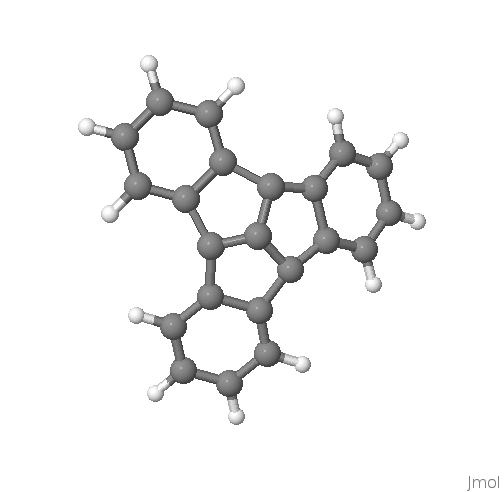
\includegraphics[scale=0.5]{M2_0001.png}\\
\begin{tabular}{c c c c}
\iffalse
SFTDDFT sp & cc-pVTZ & -845.19214555 & singlet\\
SFTDDFT sp & cc-pVTZ & -845.20881900 & triplet\\
\fi
SFTDDFT sp & cc-pVTZ & 0.45370791732958554 & singlet triplet\\
\iffalse
CAMB3LYP & cc-pVTZ & -845.238818389652 & singlet\\
CAMB3LYP & cc-pVTZ & -845.260549628641 & triplet\\
\fi
CAMB3LYP & cc-pVTZ & 0.5913374366250354 & singlet triplet gap\\
\iffalse
B3LYP & cc-pVTZ &  -845.736447057915 & singlet\\
B3LYP & cc-pVTZ &  -845.751617193667 & triplet \\
\fi
B3LYP & cc-pVTZ & 0.4128006320016161 & singlet triplet\\
\iffalse
CCSD & def2-svp & -840.85136673 & singlet\\
CCSD & def2-svp & -840.87906707 & triplet\\
\fi
CCSD & def2-svp & 0.7537650318766523 & singlet triplet \\
\end{tabular}
\linebreak
This molecule has 144 electron and in calculation while using def-svp basis set 368 basis functions were employed. The calculated ground state energy came out to be with in the range of 843 \( \pm \) 3 Hartree. Triplet optimised structure has lower energy than singlet optimised one. So molecule has triplet ground state. Thus it is biradical.\\ 
Bond distance of the central carbon from the neighbouring carbon of the singlet structure(in Angstrom)\\*
\begin{tabular}{c c}
\(c^{*}-c^{1}\) & 1.41428 \\
\(c^{*}-c^{2}\) & 1.35238 \\
\(c^{*}-c^{3}\) & 1.41430 \\
\end{tabular}\\*
Bond angle of the central carbon from the neighbouring carbon of the singlet structure (in degree)\\*
\begin{tabular}{c c}
\(c^{1}-c^{*}-c^{2}\) & 115.191\\
\(c^{2}-c^{*}-c^{3}\) & 115.192\\
\(c^{3}-c^{*}-c^{1}\) & 116.572\\
\end{tabular}\\*
Bond distance of the central carbon from the neighbouring carbon of the triplet structure\\*
\begin{tabular}{c c}
\(c^{*}-c^{1}\) 1.38887 \\
\(c^{*}-c^{2}\) 1.38871 \\
\(c^{*}-c^{3}\) 1.38887 \\
\end{tabular}\\*
Bond angle of the central carbon from the neighbouring carbon of the triplet structure (in degree)\\*
\begin{tabular}{c c}
\(c^{1}-c^{*}-c^{2}\) & 115.160 \\
\(c^{2}-c^{*}-c^{3}\) & 115.160 \\
\(c^{3}-c^{*}-c^{1}\) & 115.143 \\
\end{tabular}\\*

In the molecule the deviation of angle and and bond length is less in triplet structure in comparison with that of singlet structure.
Deviation of distance is 0.06 Angstrom and angle is 1.38 degree in singlet structure where as in triplet structure deviation of distance is 0.00016 Angstrom and of angle is 0.017 degree
\iffalse
############################################################################
#
# Molecule 2 with 3H
#
############################################################################
\fi
\pagebreak
\section{Molecule 2 with 4H}
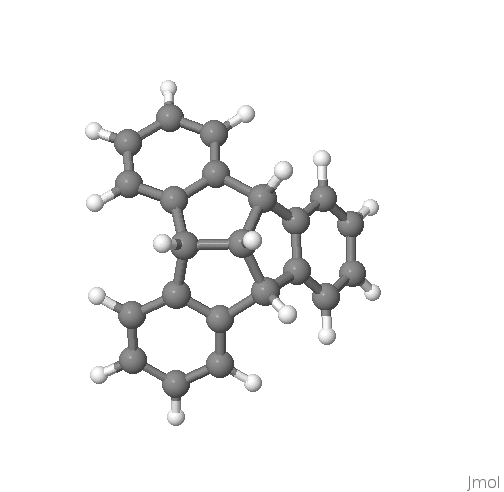
\includegraphics[scale=0.5]{M2_h_0001.png}\\
The molecule has 148 electrons and 884 basis function were used to perform CAMB3LYP calculation. The calculated ground state energy came out to be 847.78 \( \pm \) 1 hartree. Singlet optimised structure has lower energy than triplet optimised structure. To perform dft calculation on the molecular structure for triplet electronic configuration DIIS\_GDM SCF algorithm was employed as SCF convergence critaria  were not met with DIIS algorithm. Further it was not fesible to perform CCSD calculation on the structure for triplet configuration.

\begin{tabular}{c c c c}
CAMB3LYP & cc-pVTZ & -847.788744311852  & singlet\\
CAMB3LYP & cc-pVTZ & -847.651506736526  & triplet\\

CAMB3LYP & cc-pVTZ & -3.7344265572266178ev & singlet triplet gap\\
\end{tabular}\\*
Bond distance of the central carbon from the neighbouring carbon of the singlet structure(in Angstrom)\\*
\begin{tabular}{c c}
\(c^{*}-c^{1}\) & 1.55813 \\
\(c^{*}-c^{2}\) & 1.55811 \\
\(c^{*}-c^{3}\) & 1.55813 \\
\end{tabular}\\*
Bond angle of the central carbon from the neighbouring carbon of the singlet structure (in degree)\\*
\begin{tabular}{c c}
\(c^{1}-c^{*}-c^{2}\) & 107.520\\
\(c^{2}-c^{*}-c^{3}\) & 107.545\\
\(c^{3}-c^{*}-c^{1}\) & 107.520\\
\end{tabular}\\*
Bond distance of the central carbon from the neighbouring carbon of the triplet structure (in Angstrom)\\*
\begin{tabular}{c c}
\(c^{*}-c^{1}\) 1.55811 \\
\(c^{*}-c^{2}\) 2.20760 \\
\(c^{*}-c^{3}\) 2.21083 \\
\end{tabular}\\*
Bond angle of the central carbon from the neighbouring carbon of the triplet structure (in degree)\\*
\begin{tabular}{c c}
\(c^{1}-c^{*}-c^{2}\) & 107.420 \\
\(c^{2}-c^{*}-c^{3}\) & 107.391 \\
\(c^{3}-c^{*}-c^{1}\) & 107.504 \\
\end{tabular}\\*
In the molecule the deviation of angle and and bond length is less in singlet structure in comparison with that of triplet structure.
Deviation of distance is 2.0 \( \times 10^{-5} \) Angstrom and angle is 0.025 degree in singlet structure where as in triplet structure deviation of distance is 0.6527 Angstrom and of angle is 0.113 degree


\iffalse
############################################################################
#
# Molecule 3
#
############################################################################
\fi
\pagebreak
\section{Molecule 3}
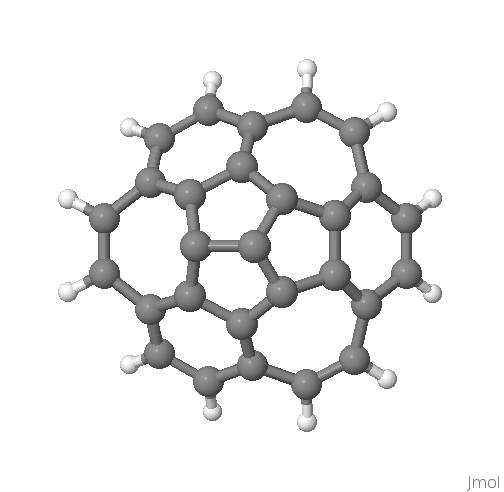
\includegraphics[scale=0.5]{M3_0001.png}\\
\begin{tabular}{c c c c}
\iffalse
SFTDDFT & cc-pVTZ & -1073.70914412 & singlet\\
SFTDDFT & cc-pVTZ & -1073.72210510 & triplet\\
\fi
SFTDDFT & cc-pVTZ & 0.3526864111689762 & singlet triplet gap\\
\iffalse
CAMB3LYP & cc-pVTZ & -1073.77169616638 & singlet\\
CAMB3LYP & cc-pVTZ & -1073.78812220792 & triplet\\
\fi
CAMB3LYP & cc-pVTZ & 0.44697558676003163 & singlet triplet gap\\
\iffalse
B3LYP & cc-pVTZ & -1074.39036244749 & singlet\\
B3LYP & cc-pVTZ & -1074.40033465399 & triplet\\
\fi
B3LYP & cc-pVTZ & 0.27135769995822295 & singlet triplet gap\\
\iffalse
CCSD & def2-svp & -1068.17916208 & singlet\\
CCSD & def2-svp & -1068.24641579 & triplet\\
\fi
CCSD & def2-svp & 1.8300676042921427 & singlet triplet\\
\end{tabular}\\*
The molecule has 180 electrons and 1008 basis functions were used for the calculation with cc-pVTZ basis function. 
Triplet ground state is lower than the singlet ground state.
Bond distance of the central carbon from the neighbouring carbon of the singlet structure(in Angstrom)\\*
\begin{tabular}{c c}
\(c^{*}-c^{1}\) & 1.40131 \\
\(c^{*}-c^{2}\) & 1.41742 \\
\(c^{*}-c^{3}\) & 1.40131\\
\end{tabular}\\*
Bond angle of the central carbon from the neighbouring carbon of the singlet structure (in degree)\\*
\begin{tabular}{c c}
\(c^{1}-c^{*}-c^{2}\) & 111.544\\
\(c^{2}-c^{*}-c^{3}\) & 111.544\\
\(c^{3}-c^{*}-c^{1}\) & 103.479\\
\end{tabular}\\*
Bond distance of the central carbon from the neighbouring carbon of the triplet structure (in Angstrom)\\*
\begin{tabular}{c c}
\(c^{*}-c^{1}\) 1.40939 \\
\(c^{*}-c^{2}\) 1.40867 \\
\(c^{*}-c^{3}\) 1.40877 \\
\end{tabular}\\*
Bond angle of the central carbon from the neighbouring carbon of the triplet structure (in degree)\\*
\begin{tabular}{c c}
\(c^{1}-c^{*}-c^{2}\) & 110.193 \\
\(c^{2}-c^{*}-c^{3}\) & 110.187 \\
\(c^{3}-c^{*}-c^{1}\) & 110.192 \\
\end{tabular}\\*
In the molecule the deviation of angle and and bond length is less in triplet structure in comparison with that of singlet structure.
Deviation of distance is 0.016 Angstrom and angle is 8.06 degree in singlet structure where as in triplet structure deviation of distance is 0.00062 Angstrom and of angle is 0.006 degree
\iffalse
############################################################################
#
# Molecule 3 with 3H
#
############################################################################
\fi
\pagebreak
\section{Molecule 3 with 4H}
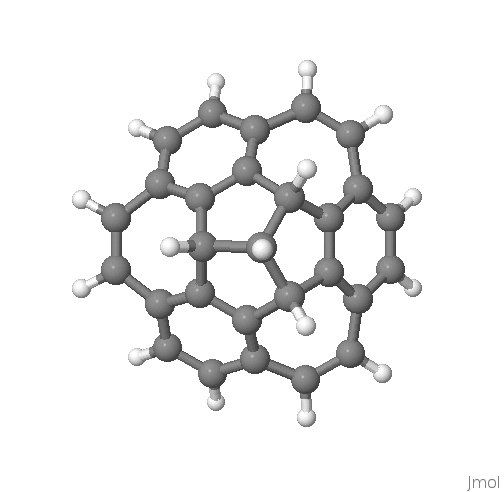
\includegraphics[scale=0.5]{M3_h_0001.png}\\
\begin{tabular}{c c c c}
\iffalse
SFTDDFT & cc-pVTZ & -1076.29343911 & singlet\\
SFTDDFT & cc-pVTZ & -1076.20719168 & triplet\\
\fi
SFTDDFT & cc-pVTZ & -2.3469133167008462 & singlet triplet\\
\iffalse
CAMB3LYP & cc-pVTZ & -1076.35294893391 & singlet\\
CAMB3LYP & cc-pVTZ & -1076.26558518342 & triplet\\
\fi
CAMB3LYP & cc-pVTZ & -2.3772899600866495 & singlet triplet\\
\iffalse
B3LYP & cc-pVTZ & -1076.96114986342 & singlet\\
B3LYP & cc-pVTZ & -1076.87924510449  & triplet\\
\fi
B3LYP & cc-pVTZ & -2.3772899600866495 & singlet triplet gap\\
\iffalse
CCSD & def2-svp & -1070.76706154 & singlet\\
CCSD & def2-svp & -1070.71796415 & triplet\\
\fi
CCSD & def2-svp & -1.3360087182471607 & singlet triplet \\
\end{tabular}\\*
Singlet ground state is lower than the triplet ground state.
Bond distance of the central carbon from the neighbouring carbon of the singlet structure(in Angstrom)\\*
\begin{tabular}{c c}
\(c^{*}-c^{1}\) & 1.55378 \\
\(c^{*}-c^{2}\) & 1.55391 \\
\(c^{*}-c^{3}\) & 1.55378\\
\end{tabular}\\*
Bond angle of the central carbon from the neighbouring carbon of the singlet structure (in degree)\\*
\begin{tabular}{c c}
\(c^{1}-c^{*}-c^{2}\) & 106.497\\
\(c^{2}-c^{*}-c^{3}\) & 106.497\\
\(c^{3}-c^{*}-c^{1}\) & 106.515\\
\end{tabular}\\*
Bond distance of the central carbon from the neighbouring carbon of the triplet structure (in Angstrom)\\*
\begin{tabular}{c c}
\(c^{*}-c^{1}\) 1.55250 \\
\(c^{*}-c^{2}\) 1.55055 \\
\(c^{*}-c^{3}\) 1.55250 \\
\end{tabular}\\*
Bond angle of the central carbon from the neighbouring carbon of the triplet structure (in degree)\\*
\begin{tabular}{c c}
\(c^{1}-c^{*}-c^{2}\) & 106.611 \\
\(c^{2}-c^{*}-c^{3}\) & 106.611 \\
\(c^{3}-c^{*}-c^{1}\) & 105.989\\
\end{tabular}\\*
In the molecule the deviation of angle and and bond length is less in singlet structure in comparison with that of singlet structure. 
Deviation of distance is 0.00013 Angstrom and angle is 0.018 degree in singlet structure where as in triplet structure deviation of distance is 0.0019 Angstrom and of angle is 0.621 degree
\iffalse
############################################################################
#
# Molecule 4
#
############################################################################
\fi
\pagebreak
\section{Molecule 4}
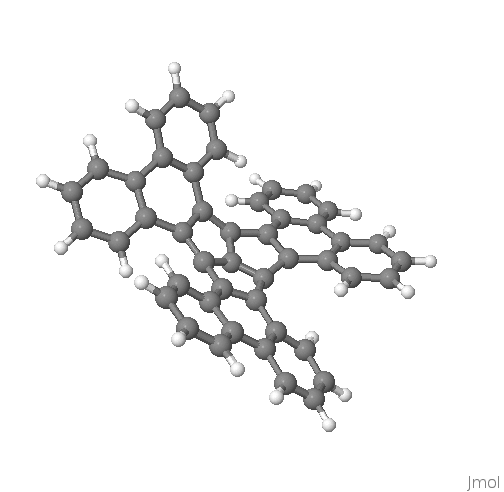
\includegraphics[scale=0.5]{M4_0001.png}\\
\begin{tabular}{c c c c}
\iffalse
SFTDDFT & cc-pVTZ & -1766.77540992 & singlet\\
SFTDDFT & cc-pVTZ & -1766.76836766 & triplet\\
\fi
SFTDDFT & cc-pVTZ & -0.19162975376222272 & singlet triplet gap\\
\iffalse
CAMB3LYP & cc-pVTZ & -1766.85968083450 & singlet\\
CAMB3LYP & cc-pVTZ & -1766.85701416889 & triplet\\
\fi
CAMB3LYP & cc-pVTZ & -0.07256370458402812 & singlet triplet gap\\
\iffalse
B3LYP & cc-pVTZ & -1767.87631324282 & singlet \\
B3LYP & cc-pVTZ & -1767.87445973020  & triplet\\
\fi
B3LYP & cc-pVTZ & -0.05043667330985882 & singlet triplet gap\\
\iffalse
CCSD & def2-svp & -1757.64842408 & singlet\\
CCSD & def2-svp & -1757.66368357 & triplet\\
\fi
CCSD & def2-svp & 0.415232086187693 & singlet triplet \\
\end{tabular}\\*
Triplet ground state is lower than the singlet ground state.
Bond distance of the central carbon from the neighbouring carbon of the singlet structure(in Angstrom)\\*
\begin{tabular}{c c}
\(c^{*}-c^{1}\) & 1.41542 \\
\(c^{*}-c^{2}\) & 1.42397 \\
\(c^{*}-c^{3}\) & 1.32505\\
\end{tabular}\\*
Bond angle of the central carbon from the neighbouring carbon of the singlet structure (in degree)\\*
\begin{tabular}{c c}
\(c^{1}-c^{*}-c^{2}\) & 116.810\\
\(c^{2}-c^{*}-c^{3}\) & 117.333\\
\(c^{3}-c^{*}-c^{1}\) & 117.551\\
\end{tabular}\\*
Bond distance of the central carbon from the neighbouring carbon of the triplet structure (in Angstrom)\\*
\begin{tabular}{c c}
\(c^{*}-c^{1}\) 1.38807 \\
\(c^{*}-c^{2}\) 1.38766 \\
\(c^{*}-c^{3}\) 1.38766 \\
\end{tabular}\\*
Bond angle of the central carbon from the neighbouring carbon of the triplet structure (in degree)\\*
\begin{tabular}{c c}
\(c^{1}-c^{*}-c^{2}\) & 114.706 \\
\(c^{2}-c^{*}-c^{3}\) & 114.707 \\
\(c^{3}-c^{*}-c^{1}\) & 114.760\\
\end{tabular}\\*
In the molecule the deviation of angle and and bond length is less in triplet structure in comparison with that of singlet structure. 
Deviation of distance is 0.09891 Angstrom and angle is 0.0.7409 degree in singlet structure where as in triplet structure deviation of distance is 0.00041 Angstrom and of angle is 0.054 degree
\iffalse
############################################################################
#
# Molecule 4 with 3H
#
############################################################################
\fi
\pagebreak
\section{Molecule 4 with 3H}
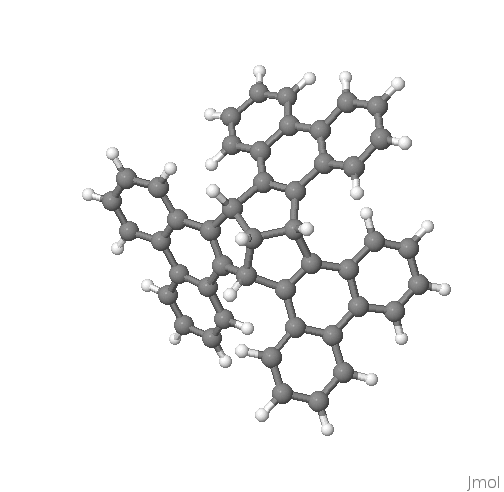
\includegraphics[scale=0.5]{M4_h0001.png}\\
\begin{tabular}{c c c c}
\iffalse
SFTDDFT & cc-pVTZ & -1769.28222770 & singlet\\
SFTDDFT & cc-pVTZ & -1769.14667471 & triplet\\
\fi
SFTDDFT & cc-pVTZ & -3.688586632084667 & singlet triplet gap\\
\iffalse
CAMB3LYP & cc-pVTZ & -1769.37294239785 & singlet\\
CAMB3LYP & cc-pVTZ & -1769.28111662713  & triplet\\
\fi
CAMB3LYP & cc-pVTZ & -2.4987077773731046 & singlet triplet gap\\
\iffalse
CCSD & def2-svp & -1760.15463826 & singlet\\
CCSD & def2-svp & calculation is still going on
\fi
\end{tabular}\\*
Singlet ground state is lower than triplet ground state.
Bond distance of the central carbon from the neighbouring carbon of the singlet structure(in Angstrom)\\*
\begin{tabular}{c c}
\(c^{*}-c^{1}\) & 1.54465 \\
\(c^{*}-c^{2}\) & 1.54518 \\
\(c^{*}-c^{3}\) & 1.54557 \\
\end{tabular}\\*
Bond angle of the central carbon from the neighbouring carbon of the singlet structure (in degree)\\*
\begin{tabular}{c c}
\(c^{1}-c^{*}-c^{2}\) & 107.824\\
\(c^{2}-c^{*}-c^{3}\) & 107.833\\
\(c^{3}-c^{*}-c^{1}\) & 107.848\\
\end{tabular}\\*
Bond distance of the central carbon from the neighbouring carbon of the triplet structure (in Angstrom)\\*
\begin{tabular}{c c}
\(c^{*}-c^{1}\) 1.55198 \\
\(c^{*}-c^{2}\) 1.54825 \\
\(c^{*}-c^{3}\) 1.55107 \\
\end{tabular}\\*
Bond angle of the central carbon from the neighbouring carbon of the triplet structure (in degree)\\*
\begin{tabular}{c c}
\(c^{1}-c^{*}-c^{2}\) & 107.479 \\
\(c^{2}-c^{*}-c^{3}\) & 107.793 \\
\(c^{3}-c^{*}-c^{1}\) & 107.285 \\
\end{tabular}\\*
In the molecule the deviation of angle and and bond length is less in singlet structure in comparison with that of singlet structure. 
Deviation of distance is 0.0009 Angstrom and angle is 0.024 degree in singlet structure where as in triplet structure deviation of distance is 0.00373 Angstrom and of angle is 0.508 degree
\iffalse
############################################################################
#
# Molecule 5
#
############################################################################
\fi
\pagebreak
\section{Molecule 5}
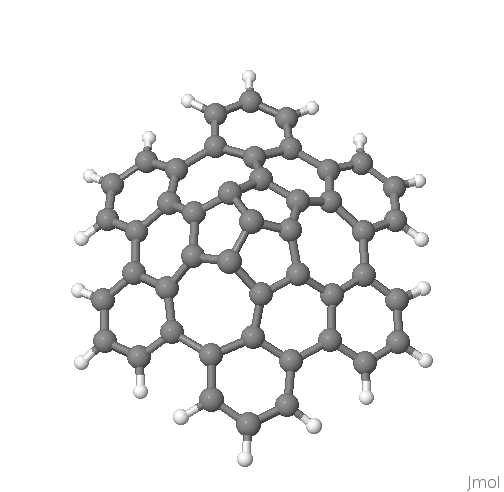
\includegraphics[scale=0.5]{M5_0001.png}\\
\begin{tabular}{c c c c}
\iffalse
SFTDDFT & cc-pVTZ & -1763.08431069  & singlet\\
SFTDDFT & cc-pVTZ &  -1763.10811358 & triplet\\
\fi
SFTDDFT & cc-pVTZ & 0.6477099609479039 & singlet triplet gap\\
\iffalse
CAMB3LYP & cc-pVTZ &  -1763.19618198736 & singlet\\
CAMB3LYP & cc-pVTZ & -1763.19647589922 & triplet\\
\fi
CAMB3LYP & cc-pVTZ & 0.007997753190637332 & singlet triplet gap\\
\iffalse
B3LYP & cc-pVTZ & -1764.19642372060 & singlet\\
B3LYP & cc-pVTZ & -1764.19660214816 & triplet\\
\fi
B3LYP & cc-pVTZ & 0.004855263707775339 & singlet triplet gap\\

\end{tabular}\\*

Singlet ground state and Triplet ground state is degenerate.
Bond distance of the central carbon from the neighbouring carbon of the singlet structure(in Angstrom)\\*
\begin{tabular}{c c}
\(c^{*}-c^{1}\) & 1.41971 \\
\(c^{*}-c^{2}\) & 1.37285 \\
\(c^{*}-c^{3}\) & 1.41971 \\
\end{tabular}\\*
Bond angle of the central carbon from the neighbouring carbon of the singlet structure (in degree)\\*
\begin{tabular}{c c}
\(c^{1}-c^{*}-c^{2}\) & 107.248\\
\(c^{2}-c^{*}-c^{3}\) & 107.248\\
\(c^{3}-c^{*}-c^{1}\) & 110.817\\
\end{tabular}\\*
Bond distance of the central carbon from the neighbouring carbon of the triplet structure (in Angstrom)\\*
\begin{tabular}{c c}
\(c^{*}-c^{1}\) 1.40296 \\
\(c^{*}-c^{2}\) 1.40638 \\
\(c^{*}-c^{3}\) 1.40296 n\\
\end{tabular}\\*
Bond angle of the central carbon from the neighbouring carbon of the triplet structure (in degree)\\*
\begin{tabular}{c c}
\(c^{1}-c^{*}-c^{2}\) & 108.797 \\
\(c^{2}-c^{*}-c^{3}\) & 108.767 \\
\(c^{3}-c^{*}-c^{1}\) & 108.524 \\
\end{tabular}\\*
In the molecule the deviation of angle and and bond length is less in triplet structure in comparison with that of singlet structure. 
Deviation of distance is 0.0466 Angstrom and angle is 3.56 degree in singlet structure where as in triplet structure deviation of distance is 0.0034 Angstrom and of angle is 0.273 degree

\section{Conclusion}

The molecular structure which is derived from acepentalene has its triplet structure optimised for triplet state has its ground state energy lower than the ground state energy of structure optimised for singlet except for acepentalene. That implies existence of these molecules in biradical form. Also though DFT calculation for acepentalene shows it's singlet ground state is lower, but CCSD calculation shows that it has lower triplet state. Also as shown in previous report acepentalene have biradicaloid charecter 

Hydeogenated acepentalene derivative have a lower singlet than triplet. 

Based on the deviation data of angles and of distance of central carbon to its neighbouring carbon. It is inferred that the structure with lower energy has less deviation. And So it is more symmetric. 
\fi

\bibliographystyle{unsrt}

\bibliography{anurag}

\end{document}
